\chapter{情绪障碍和焦虑} \label{chap:chap61}

自古以来,抑郁症、躁郁症和焦虑症在医学著作中都有详细记载。 
在公元前五世纪,\textit{希波克拉底}教导说,情绪取决于四种体液:血液、痰、黄胆汁和黑胆汁的平衡。
过量的黑胆汁(忧郁症是古希腊语中黑胆汁的称呼)被认为会导致恐惧和沮丧。
\textit{罗伯特$\cdot$波顿}的《忧郁的解剖》不仅是一本重要的医学著作,而且还通过忧郁症的视角来看待文学和艺术。
这些文字描述的症状在今天仍然很熟悉;
他们还认识到抑郁症和焦虑症的症状经常同时发生。


在本章中,我们一起讨论情绪障碍和焦虑症,这不仅是因为它们经常同时发生,而且还因为重叠的遗传和环境风险因素以及一些共同的神经结构,包括杏仁核、海马体、前额叶皮层和岛叶皮层区域。



\section{情绪障碍可分为两大类:单相抑郁症和双相情感障碍}

目前还没有针对情绪障碍和焦虑障碍的客观医学测试。
因此,诊断取决于对症状、行为、认知、功能障碍和自然病程(包括发病年龄、病程和结果)的观察。
家族传播模式和对治疗的反应也可以为诊断分类提供信息。
基于这些因素,可以区分两大类情绪障碍:单相抑郁症和双相情感障碍。
单相抑郁症,当严重且普遍时,被归类为\textit{重度抑郁症}。
当人们单独遭受抑郁发作时,可诊断为\textit{重度抑郁症}。
当躁狂发作也发生时,双相情感障碍就被诊断出来了。


在美国,\textit{重度抑郁症}的终生风险约为 19\%。
在任何 1 年期间内,8.3\% 的人口患有\textit{重度抑郁症}。
不同国家和文化的抑郁症患病率不同;
然而,在缺乏客观医学检测的情况下,此类流行病学数据存在诊断和报告偏差,因此很难得出比较结论。
世界卫生组织报告说,抑郁症是全世界残疾的主要原因,其他研究发现它是非传染性疾病造成经济损失的主要原因。
这些可怕的社会和经济后果的发生是因为抑郁症很常见,通常在生命早期开始,并且会干扰认知、精力和动机,而这些都是在学校学习和有效工作所必需的。


双相情感障碍不如单相抑郁症常见,全球患病率约为 1\%。
它的症状在各个国家和文化中都相对稳定。
双相情感障碍的发病率在男性和女性中相当。



\subsection{\textit{重度抑郁症}与正常的悲伤有很大不同}

有几个因素可以将\textit{重度抑郁症}与日常生活中可能出现的短暂悲伤时期以及通常在个人损失后的悲伤区分开来。
这些包括症状发生的生活环境、持续时间和普遍性,以及它们与生理、行为和认知症状的关联(表~\ref{tab:61_1})。
在健康人中,情绪在低和高之间交替,时间和强度与人际交往和生活事件相适应。
根据情境不当、幅度极端、僵化或持续时间长的情绪状态,根据它们的效价,提示抑郁症或躁狂症。


\begin{table}[htbp]
	\caption{情绪障碍的症状~\cite{vahia2013diagnostic} \label{tab:61_1}}
	\begin{tabular}{l}
		\toprule
		\makecell[l]{在同一个两周内出现了以下五种或五种以上症状,这代表了与以前功能的变化。
		至少有一种症状是(1) \\情绪低落或(2)失去兴趣或快乐。} \\
		\midrule
		\makecell[l]{1. 一天中的大部分时间,几乎每天都是抑郁的情绪,无论是主观报告(如感到悲伤、空虚、绝望)还是其\\他人的观察(如看起来泪流满面)都表明了这一点。}\\
		\makecell[l]{2. 在一天中的大部分时间,几乎每天,对所有或几乎所有活动的兴趣或乐趣明显减弱(如他人的主观描述或\\观察所示)。}\\
		\makecell[l]{3. 不节食时体重显著减轻,或体重增加(例如,一个月内体重变化超过5\%),或食欲几乎每天都在下降\\或增加。}\\
		4. 几乎每天都失眠或嗜睡。\\
		5. 精神运动激动或迟钝几乎每天都有(其他人可以观察到,而不仅仅是主观上的不安或被放慢的感觉)。  \\
		6. 几乎每天都感到疲劳或精力不足。\\
		7. 几乎每天都有毫无价值或过度或不适当的内疚感(这可能是妄想)(不仅仅是对生病的自责或内疚)。\\
		8. 几乎每天都在思考或集中注意力的能力下降,或犹豫不决(无论是主观解释还是其他人观察到的)。\\
		\makecell[l]{9. 反复出现的死亡念头(不仅仅是对死亡的恐惧),没有具体计划的反复出现的自杀意念,或自杀未遂\\或自杀的具体计划。} \\
		\bottomrule
	\end{tabular}
\end{table}


抑郁发作,无论是与单相还是双相疾病相关,都以消极的情绪状态为特征,例如悲伤、焦虑、兴趣丧失或烦躁持续一天的大部分时间,日复一日,并且以前愉快的事件无法缓解。
哈姆雷特的抱怨很好地表达了这种兴趣的丧失,“人世间的一切在我看来是多么令人厌倦、陈腐、枯燥而无聊啊!” 
当抑郁症严重时,个人可能会遭受强烈的精神痛苦和普遍无法体验快乐,这种情况称为快感缺失。


抑郁症的生理症状包括睡眠障碍,最常见的是失眠和早醒,但偶尔也会过度睡眠;
食欲不振和体重减轻,但偶尔会暴饮暴食;
对性活动的兴趣下降;
和精力不足。
一些受严重影响的人表现出运动速度减慢,被描述为精神运动迟缓,而其他人可能会激动,表现出诸如来回踱步等症状。
认知症状在思想内容(绝望、无价值感和内疚感、自杀念头和冲动)和认知过程(注意力不集中、思维迟缓和记忆力差)中都很明显。


在最严重的抑郁症病例中,可能会出现精神病症状,包括妄想(无法用一个人的文化来解释不可动摇的错误信念)和幻觉。
当抑郁症出现精神病症状时,它们通常反映了该人认为自己不值得、毫无价值或不好的想法。
例如,一个严重抑郁的人可能会认为他正在散发强烈的气味,因为他正在从内部腐烂。


抑郁症最严重的后果是自杀,这是全世界死亡的一个重要原因;
世界卫生组织估计每年有 80 万人死于自杀。
超过 90\% 的自杀与精神疾病有关,抑郁症是主要的危险因素,尤其是当伴有物质使用障碍时。



\subsection{\textit{重度抑郁症}通常在生命早期开始}

\textit{重度抑郁症}通常在生命早期开始,但第一次发作确实会贯穿整个生命周期。
那些在童年或青春期首次发作的人通常有这种疾病的家族史,并且复发的可能性很高。
一旦发生第二次发作,通常会出现反复复发和缓解的模式。
有些人不会从急性发作中完全恢复,而是患有慢性抑郁症,尽管较轻,但可能会因急性加重而间歇性发作。
慢性抑郁症,即使症状没有急性发作那么严重,也可能因为长期侵蚀一个人在生活中发挥作用的能力而极其致残。
儿童期\textit{重度抑郁症}在男性和女性中的发生率相同。
然而,在青春期之后,它更常见于女性;
在不同国家和文化中,女性与男性的比例约为 2:1。



\subsection{双相情感障碍的诊断需要躁狂发作}

双相情感障碍因其主要症状而得名,情绪在躁狂和抑郁之间摇摆不定;
事实上,19 世纪颇具影响力的精神病学家\textit{埃米尔$\cdot$克雷佩林}将这种情况称为躁郁性精神错乱。
按照惯例,双相情感障碍的诊断需要至少有一次躁狂发作。
躁狂症通常与反复发作的抑郁症有关,而没有抑郁症的躁狂症则明显不常见。


躁狂发作的典型特征是情绪高涨,尽管有些人主要是易怒。
在躁狂发作期间,个体的能量显著增加,睡眠需求减少,偶尔食欲下降(表~\ref{tab:61_2})。
患有躁狂症的人通常是冲动的,并且过度地从事以奖赏为导向的行为,通常以极度乐观为特征的判断力差。
例如,一个人可能会继续疯狂消费,远远超出他或她的能力范围,或者出现异常的药物和酒精使用或性行为狂欢。
自尊心通常被夸大,常常达到妄想的程度。
例如,一个人可能错误地认为自己对事件具有广泛的影响力或是重要的宗教人物。 在古代,躁狂症被描述为“一种情绪高涨的疯狂状态”。
然而,这种高涨的情绪可能是脆弱的,伴随着愤怒、易怒和攻击性的突然闯入。


\begin{table}[htbp]
	\caption{躁狂发作的症状~\cite{vahia2013diagnostic} \label{tab:61_2}}
	\begin{tabular}{l}
		\toprule
		\makecell[l]{A. 一段明显的异常和持续的情绪高涨、膨胀或易怒,以及异常和持续增加的目标活动或能量,持续至少 1 \\周(或任何持续时间,如果需要住院治疗)。 }\\
		\makecell[l]{B. 在情绪紊乱和精力或活动增加期间,以下三种(或更多)症状(如果情绪只是易怒,则为四种)持续\\存在,并在很大程度上存在:} \\
		1. 自负或浮夸。\\
		2. 睡眠需求减少(例如,只睡了 3 个小时就感到休息了)。\\
		3. 比平时更健谈或有压力继续说话。\\
		4. 思想的逃亡或主观经验,认为思想在飞速发展。 \\
		5. 注意力分散(即注意力太容易被不重要或无关的外部刺激所吸引)。\\
		6. 目标导向活动(社交、工作、学校或性行为)或心理运动激动(即无目的的非目标导向活动)的增加。 \\
		7. 过度参与有可能带来痛苦后果的愉快活动(如无节制的疯狂购买、性行为不检点或愚蠢的商业投资)。 \\
		\bottomrule
	\end{tabular}
\end{table}


躁狂症与抑郁症一样,会影响认知过程,通常会损害注意力和语言记忆。
在躁狂发作期间,一个人的讲话通常是快速、冗长且难以打断的。
这个人可能会从一个想法跳到另一个想法,使言语理解变得困难。
精神病症状通常发生在躁狂发作期间,并且通常与人的情绪一致。
例如,患有躁狂症的人可能会妄想拥有特殊的力量或成为奉承的对象。


双相情感障碍中发生的抑郁发作在症状上与单相抑郁症无法区分,但往往更难治疗。
例如,他们通常对抗抑郁药物的反应较差。
纵向研究发现,躁郁症患者在严重的躁狂症或抑郁症急性发作之间最常见的情感状态并不是旧教科书中经常教导的健康情绪(幸福感),而是一种慢性抑郁症状态。


从历史上看,双相情感障碍的概念描述的是经历过完全躁狂发作的患者,这些发作通常包括精神病症状和必要的住院治疗(表~\ref{tab:61_2})。
近几十年来,诊断分类增加了 2 型双相情感障碍,其中轻度躁狂(也称为轻躁狂)与抑郁发作交替出现。
根据定义,2 型双相情感障碍的躁狂发作不伴有精神病或严重到需要住院治疗。
这是否代表经典(1 型)双相情感障碍或某些其他病理生理学的变体尚不清楚,尽管情绪障碍的基因解剖可能会在不久的将来提供一些澄清。


双相情感障碍通常开始于年轻的成年期,但发病时间可能早于或晚至 50 岁。
许多躁狂发作往往缺乏明显的诱因;
然而,睡眠剥夺会引发某些躁郁症患者的躁狂发作。
对于这些人来说,跨时区旅行或轮班工作是一种风险。
双相情感障碍患者的躁狂、抑郁和正常情绪周期之间的循环率差异很大。
周期短、周期快的人往往对情绪稳定药物的反应较差。



\section{焦虑症代表恐惧回路的显著失调}

焦虑症是全世界最常见的精神疾病。
在美国,28.5\% 的人口在其一生中患有一种或多种焦虑症。
一些焦虑症是轻微的,例如涉及很少遇到的刺激的简单恐惧症;
其他人,如恐慌症或创伤后应激障碍,根据症状的严重程度、功能障碍和长期性,通常会非常虚弱。


焦虑和恐惧是相关的情绪状态;
两者对于在一生中可能遇到的危险中幸存下来都至关重要。
主要区别在于恐惧是对存在的威胁的反应,并且明显表示危险,而焦虑是对威胁的准备状态,这些威胁在接近度或时间上都不那么具体。
恐惧和焦虑的神经回路强烈重叠,它们的生理、行为、认知和情感方面也是如此。


恐惧通常是对危险的短暂适应性反应,就像疼痛一样,是一种生存机制。
像疼痛一样,恐惧是警觉和厌恶的,并或多或少地激发立即的行为反应。
因此,恐惧会打断正在进行的行为,用回避或防御性攻击等反应取代它们。
为了让身体做好生理应对的准备,恐惧回路会激活交感神经系统并导致压力荷尔蒙的释放。
这种“战斗或逃跑”反应促进血液流向骨骼肌,增加新陈代谢活动,并提高疼痛阈值。
与奖励和其他与生存相关的情绪反应一样,恐惧强烈地促进了内隐和外显记忆的编码和巩固,这些记忆使有机体能够快速有效地对未来的预测线索做出反应。 
(恐惧回路在第~\ref{chap:chap42}~章中描述。)


焦虑的许多认知和生理成分与恐惧相似,但通常表现出较低的强度和较长的时间进程。
当与威胁的可能性和可能的严重程度成比例时,焦虑是适应性的,从而导致适当水平的唤醒、警惕和生理准备。
鉴于忽视甚至是模棱两可的威胁线索的危险,甚至可能致命的后果,未能做出适当的焦虑反应可能被证明是高度适应不良的。
然而,过度的情境不适当和长时间的警惕、紧张和生理激活可能是令人痛苦和致残的焦虑症或可能伴随抑郁症的焦虑症状的基础。
焦虑症的危险因素包括一个人的遗传背景、发育经历,以及不仅来自直接经验而且来自家庭、同龄人、学校和其他机构的教训。


引起焦虑的线索可能是环境的或内感受的(即来自身体内部,例如腹部不适或心悸)。
社交暗示和社交情境可能是焦虑的主要来源。
在人类中,焦虑状态也可以由引发对危险的记忆或想象的思路引发。
焦虑也可能源于由于其简洁或模糊而被无意识地处理的刺激,并且由此产生的情绪可能会被体验为自发产生的。
与由表示威胁的明确刺激的存在或终止而引发和终止的恐惧相反,焦虑具有更多变的时间进程。
如果危险或伤害的可能性持续很长时间,或者没有明确的安全信号,焦虑状态可能会延长。


焦虑症和可能伴随\textit{重度抑郁症}的焦虑与多种症状相关。
受影响的个人可能会过度关注可能的威胁和对被解释为威胁的线索的注意偏见。
这种认知状态通常与持续的担忧、紧张和警惕有关。
常见的生理症状包括过度警觉,表现为惊吓阈值低、睡眠困难和交感神经系统激活,包括快速、剧烈的心跳。
患有焦虑症的人可能会非常清楚地意识到自己的心跳或呼吸,这本身就可能成为全神贯注和担忧的来源。
在惊恐发作期间,交感神经系统的激活可能达到极端强度,这是焦虑最严重的表现之一。


在焦虑症中,面对严重威胁时会适应的认知、生理和行为反应可能会被无害刺激不适当地激活,可能对情况不适当地强烈,并且可能有一个安全信号失效的长期过程 终止症状。
受影响的个人可能会避开一些地方、人或经历,这些地方、人或经历虽然客观上是安全的,但与威胁的感知或焦虑的经历有关。
严重时,这种回避会损害受影响的个人以不同的能力或角色发挥作用的能力。


由于没有针对特定焦虑症状群的生物标志物或客观医学测试,当前的精神病学分类,例如精神疾病诊断和统计手册(第五版),根据临床病史对焦虑症进行分类,例如性质 、强度和症状的时间过程、外部线索在触发事件中的作用以及相关症状。
精神疾病诊断和统计手册(第五版)将病理性焦虑症分为几种不同的疾病:恐慌症、创伤后应激障碍、广泛性焦虑症、社交焦虑症(以前称为社交恐惧症)和单纯性恐惧症。
出于启发式目的,这些障碍将在下文讨论,但目前来自长期临床观察和家庭、双胞胎和流行病学研究的证据不支持将焦虑症状分为离散的非重叠类别。
相反,证据表明,病理性焦虑症状和抑郁症状可能更好地概念化为连续体或光谱,其中个体经历跨越当前 精神疾病诊断和统计手册边界的不同症状。


与症状谱的概念一致,焦虑症和抑郁症并不经常作为不同的精神疾病诊断和统计手册(第五版)类别在家庭中跨代同时发生;
相反,在受影响的家庭成员中通常会观察到不同模式的焦虑和抑郁症状。
比较同卵双胞胎和异卵双胞胎特征一致性的双胞胎研究发现,多种焦虑症和\textit{重度抑郁症}之间存在显著的共同遗传风险。
此外,流行病学研究发现,被诊断患有一种明确的精神疾病诊断和统计手册(第五版)焦虑症的人,例如在青少年时期,很有可能在未来十年内出现新的焦虑或抑郁症状,这可能导致该人被诊断出患有基于精神疾病诊断和统计手册(第五版)分类的多种疾病。
推定不同的精神疾病诊断和统计手册(第五版)焦虑症和抑郁症同时发生的高频率以及家庭和双胞胎研究的结果表明,焦虑症和\textit{重度抑郁症}之间存在显著共享的病因和致病机制。
尽管如此,下面简要描述了精神疾病诊断和统计手册(第五版)中列出的个别疾病。


惊恐发作是焦虑的严重表现。
它们的特点是不连续的(可以持续很多分钟)强烈的不祥预感、厄运感、害怕失去对自己的控制或害怕死亡。
它们与显著的身体症状有关,例如心悸、呼吸困难、出汗、感觉异常和头晕(表~\ref{tab:61_3})。


\begin{table}[htbp]
	\caption{躁狂发作的症状~\cite{vahia2013diagnostic} \label{tab:61_3}}
	\begin{tabular}{l}
		\toprule
		\makecell{一段离散的强烈恐惧或不适期,在此期间,以下四种(或多种)症状突然出现,并在 10 分钟内达到峰值。} \\
		1. 心悸、心跳加快或心率加快;\\
		2. 出汗;\\
		3. 颤抖;\\
		4. 呼吸急促或窒息感;\\
		5. 感到窒息; \\
		6. 胸痛或不适;\\
		7. 恶心或腹部不适 \\
		8. 感到头晕、不稳定、头晕或头晕 \\
		9. 冷或热的感觉;\\
		10. 感觉异常(麻木或刺痛感)\\
		11. 脱现实(感觉或不真实)或人格解体(脱离自我);\\
		12. 害怕失去控制或“发疯”;\\
		13. 对死亡的恐惧;\\
		\bottomrule
	\end{tabular}
\end{table}


惊恐发作通常会引起对未来发作的焦虑,以至于发生发作的环境可能会变成引发后续发作的恐惧刺激(恐惧条件反射)。
因此,一些受到严重影响的人会限制他们的活动,以避免发生惊恐发作或他们担心一旦遭受袭击可能无法逃脱的情况或地点。
受影响最严重的人可能会出现普遍的恐惧回避,导致他们足不出户,这种状态被称为广场恐惧症。
当前的诊断分类系统(例如精神疾病诊断和统计手册第五版)根据发作的次数和频率以及是否可以识别恐惧触发因素来定义恐慌症。
如此详细的标准缺乏强有力的经验基础,但可以肯定的是,反复出现惊恐发作和其他焦虑症状的人不仅非常痛苦,而且可能严重残疾。


\textit{创伤后应激障碍}是在经历了严重的危险或受伤之后出现的。
根据不同的名称和描述,包括第一次世界大战期间创造的术语\textit{战斗疲劳症},创伤后应激障碍长期以来一直被认为是战斗的结果。
最近,平民创伤,如袭击、强奸或车祸,已被认为是创伤后应激障碍的潜在原因。
目前针对创伤后应激障碍的方法是由美国精神病学协会根据越战退伍军人的经验正式确定的。


创伤后应激障碍是由创伤经历引发的。
其主要症状包括创伤事件的侵入性再体验,通常由声音、图像或其他创伤提示等线索引发。
例如,一个被殴打的人可能会对来自背后的意想不到的触摸做出强烈反应。
此类发作通常以交感神经系统激活为特征,严重时可能以“战斗或逃跑”反应为特征。
创伤性事件的重新体验也可能以噩梦的形式发生。
创伤后应激障碍的其他症状包括可能会干扰人际关系和社交互动的情绪麻木、失眠、慢性过度警觉(包括过度警惕)、交感神经系统激活,以及对触摸或声音等无害刺激的过度惊吓反应。


\textit{广泛性焦虑障碍}是在一个人长期担心和警惕情况不合理时被诊断出来的。
这种担忧伴随着生理症状,例如交感神经系统激活增强和运动紧张。
广泛性焦虑障碍通常与\textit{重度抑郁症}同时发生。


\textit{社交焦虑症}的特征是对社交场合的持续恐惧,尤其是当一个人受到他人审视的场合。
受影响的人非常害怕以一种会被证明是羞辱的方式行事。
怯场是社交焦虑的一种形式,仅限于表演环境,例如公开演讲。
社交焦虑障碍会导致避免在课堂上口头参与或在工作中与他人交流,因此可能会导致残疾和痛苦。



\textit{简单恐惧症}包括对特定刺激的强烈和不恰当的过度恐惧,例如电梯、飞行、高处或蜘蛛。



\section{遗传和环境风险因素都会导致情绪和焦虑症}

双相情感障碍、\textit{重度抑郁症}和焦虑症都在家族中遗传。
比较同卵双胞胎和异卵双胞胎的一致性率的双胞胎研究表明,这些疾病具有显著的遗传性,其中遗传性由遗传变异解释表现型变异的百分比来表示。
在心境障碍和焦虑障碍中,双相情感障碍的遗传性最高(70\%至80\%);
\textit{重度抑郁症}和焦虑症表现出较低但仍然显著的遗传性(约 35\%),发育和环境风险因素的作用更大。
尽管基因在情绪障碍和焦虑症的发病机制中起着重要作用,但它们都表现出非孟德尔遗传模式的跨代传播,包括\textit{重度抑郁症}和焦虑症的频繁同时发生。
这种模式反映了遗传和非遗传风险因素的复杂性。


旨在发现易患情绪和焦虑症的精确脱氧核糖核酸序列变异(等位基因)的分子遗传学研究已经启动。
此类研究具有挑战性,因为这些以及实际上所有常见精神疾病的风险结构是高度多基因的,这意味着人口风险似乎涉及与数百个基因相关或包含在数百个基因中的数千个常见和罕见等位基因。
与亨廷顿病等一些神经系统疾病不同,不存在“抑郁基因”或“焦虑基因”。
与疾病相关的等位基因对疾病风险产生小的累加效应。
任何给定个体的风险都来自与发育和环境因素协同作用的遗传负荷(由与疾病相关的等位基因的不同组合组成)。
这种多基因结构解释了非孟德尔传播模式以及在家庭和人群中观察到的抑郁和焦虑症状的不同组合。


缺乏对情绪和焦虑症的客观诊断测试意味着任何研究队列都可能有一定比例的诊断错误分类。
因此,通过\textit{全基因组关联研究}搜索常见疾病相关变异和通过脱氧核糖核酸测序搜索罕见疾病相关变异需要非常大的队列和跨多个队列进行的荟萃分析所赋予的显著统计能力。
\textit{重度抑郁症}和双相情感障碍的\textit{全基因组关联研究}早期结果已有报道;
在这两种情况下,迄今为止已经发现了几个重要的全基因组位点,但还不足以确定发病机制的分子途径。
全外显子组测序(即编码蛋白质的所有基因组区域的脱氧核糖核酸测序)和全基因组测序正在针对双相情感障碍进行。


情绪障碍和焦虑症的高度多基因风险结构意味着测试可能与这些疾病相关的一个或几个风险基因变异没有诊断价值。
相反,\textit{多基因风险评分}基于一个性状的所有遗传风险变异的总和,正在成为流行病学和临床研究中根据遗传风险严重程度对个体进行分层的有用工具。
临床队列中有差异的\textit{多基因风险评分},例如,在对\textit{重度抑郁症}患者的研究中显示低抑郁症风险,将表明错误分类。
需要强调的是,情绪障碍和焦虑症风险的多基因性质以及环境风险因素的重要贡献意味着,与任何基因测试一样,\textit{多基因风险评分}仅提供概率。


随着越来越多的了解,\textit{多基因风险评分}可以与其他措施相结合,以产生更具预测性的风险评分,就像现代心脏风险模型越来越多地包括遗传措施、吸烟史、血脂水平和血压一样。
对于情绪障碍和焦虑症,一种显示出早期希望的措施是识别源自静息状态\textit{功能性磁共振成像}(当受试者不从事任务表现时进行的成像)的神经连接的内在模式。
不同的连接模式可能会区分不同形式的障碍。


流行病学证据已经确定了严重抑郁症和焦虑症的重要发育危险因素。
最好的记录是生命早期的身体或性虐待史、严重的儿童忽视史或其他早期严重的压力源。
对此类早期应激源的研究集中于改变\textit{下丘脑-垂体-肾上腺}轴反应性的可能作用。
对动物模型早期应激的研究表明,基因表达的表观遗传调控可能在改变发育轨迹方面发挥作用。
由于无法接触到人脑组织,因此无法轻易在人类身上对这些结果进行后续研究,因此仍然是假设性的。


抑郁症和焦虑症的其他危险因素包括酒精和其他物质使用障碍以及其他精神障碍,例如注意力缺陷多动障碍、学习障碍和强迫症。
还有证据表明,自我治疗抑郁症或焦虑症的错误尝试可能会引发酒精中毒和其他药物滥用障碍,进而使潜在的状况恶化。


可能引发新的抑郁或焦虑发作的环境因素包括生活转变,例如结婚、新工作或退休。
严重的疾病,无论是急性的还是慢性的,也与严重抑郁症和焦虑症的发作有关。
一些神经系统疾病与抑郁症的风险增加有关,包括帕金森病、阿尔茨海默病、多发性硬化症和中风。
一些处方药,如干扰素,也经常引发抑郁症。
当\textit{重度抑郁症}伴有 2 型糖尿病或心血管疾病等慢性疾病时,由于抑郁症的生理效应,例如应激激素释放增加(见下文)和参与动机降低,整体医疗结果会更差 在康复方案中。



\section{抑郁和压力共享重叠的神经机制}

抑郁和对压力的反应表现出复杂但重要的相互作用。
如前所述,严重的童年逆境是抑郁症的发展风险因素;
此外,抑郁发作可能是由压力经历引发的。
相反,抑郁症的经历本身就是有压力的,因为它会造成痛苦,并对功能产生负面影响。
从症状上看,抑郁症与慢性压力有一些共同的生理特征,包括食欲、睡眠和精力的变化。
\textit{重度抑郁症}和慢性压力都与\textit{下丘脑-垂体-肾上腺}轴的持续激活有关(图~\ref{fig:61_1})。


\begin{figure}[htbp]
	\centering
	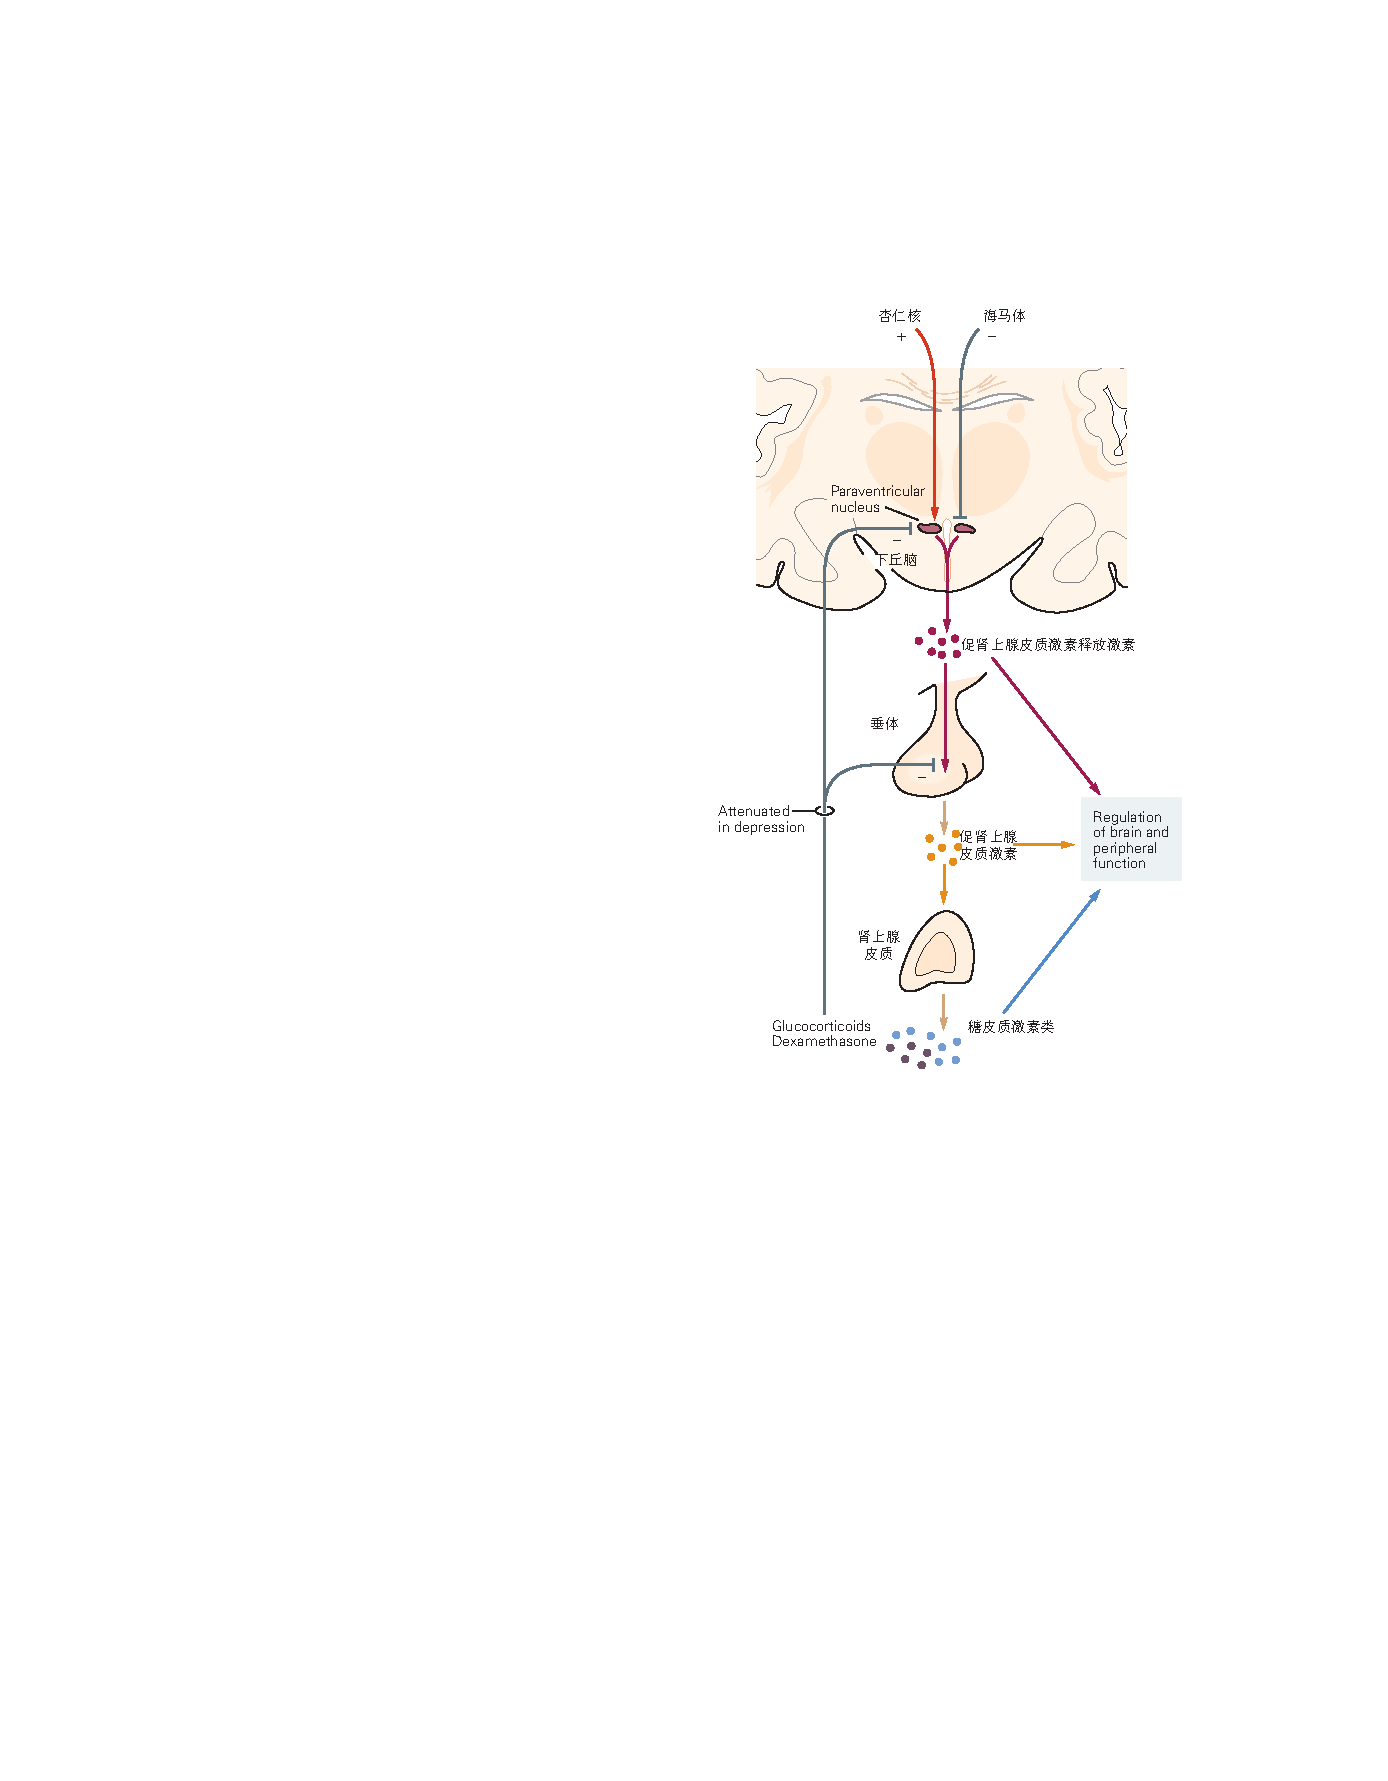
\includegraphics[width=0.6\linewidth]{chap61/fig_61_1}
	\caption{下丘脑-垂体-肾上腺轴。
		下丘脑室旁核中的神经元合成并释放\textit{促肾上腺皮质激素释放激素},这是应激激活的激素级联中的关键调节肽。
		\textit{促肾上腺皮质激素释放激素}神经元具有分泌的昼夜节律模式,应激对\textit{促肾上腺皮质激素释放激素}合成和分泌的刺激作用叠加在这种基础昼夜节律模式上。
		来自杏仁核的兴奋性纤维传递有关激活\textit{促肾上腺皮质激素释放激素}神经元的压力刺激的信息;
		抑制纤维从海马下降到室旁核。
		\textit{促肾上腺皮质激素释放激素}进入垂体门脉系统并刺激垂体前叶中合成和释放\textit{促肾上腺皮质激素}的促肾上腺皮质激素细胞。
		释放的\textit{促肾上腺皮质激素}进入体循环并刺激肾上腺皮质释放糖皮质激素。
		在人类中,主要的糖皮质激素是皮质醇;
		在啮齿动物中,它是皮质酮。
		皮质醇和合成糖皮质激素如地塞米松均在垂体和下丘脑水平起作用,分别抑制\textit{促肾上腺皮质激素}和\textit{促肾上腺皮质激素释放激素}的进一步释放。
		糖皮质激素的反馈抑制在\textit{重度抑郁症}和双相情感障碍的抑郁期减弱\cite{nestler2020nestler}。}
	\label{fig:61_1}
\end{figure}


许多但不是所有患有\textit{重度抑郁症}的人和许多处于双相情感障碍抑郁期的人表现出糖皮质激素应激激素皮质醇及其调节因子、\textit{促肾上腺皮质激素释放激素}和\textit{促肾上腺皮质激素}的过度合成和分泌。
在健康状态下,皮质醇分泌的短暂增加,如对急性压力的反应,将身体转变为分解代谢状态(使葡萄糖可用于应对压力源或威胁),增加主观能量水平,提高认知能力,并可能增加信心。
然而,糖皮质激素的长期增加可能会导致抑郁样症状。
例如,许多患有库欣病(垂体肿瘤分泌过量\textit{促肾上腺皮质激素},导致皮质醇过多)的人会出现抑郁症状。


\textit{下丘脑-垂体-肾上腺}轴内的反馈机制通常允许皮质醇(或外源性糖皮质激素)抑制\textit{促肾上腺皮质激素释放激素}和\textit{促肾上腺皮质激素}分泌,从而抑制额外的皮质醇合成和分泌。
在大约一半的\textit{重度抑郁症}患者中,这种反馈系统受损;
它们的\textit{下丘脑-垂体-肾上腺}轴甚至可以抵抗强效合成糖皮质激素(如地塞米松)的抑制。
尽管\textit{下丘脑-垂体-肾上腺}轴的容易测量的紊乱尚未证明足够敏感或特异以用作抑郁症的诊断测试,但观察到的异常强烈表明病理激活的应激反应通常是抑郁症的重要组成部分。


压力与抑郁症的关系导致在啮齿动物抑郁症模型中发展出几种慢性压力范例。
观察到许多抗抑郁药可逆转这些动物的应激引起的生理或行为变化,从而加强了这些动物模型对应激引起的综合症的依赖。
然而,动物承受各种慢性应激源的程度实际上如何模拟人类抑郁症的疾病机制仍然未知。
尽管经过 50 多年的尝试,但仍未能确定新的抗抑郁机制,这表明人们担心过度依赖基于压力的模型和其他啮齿动物模型。
使用此类模型进行的药物筛选仅识别出与原型抗抑郁药物作用相似的分子,这些药物最初是通过对人类产生意想不到的精神作用而被识别出来的。



\section{可以通过神经影像学识别与情绪和焦虑症有关的人脑结构和回路的功能障碍}

对涉及情绪和焦虑症的人脑区域和神经回路的研究依赖于非侵入性结构和功能神经影像学、神经生理学测试和尸检分析。
最近,正在从接受深部脑刺激治疗的患者的神经影像学中收集信息。



\subsection{识别功能异常的神经回路有助于解释症状并可能提出治疗建议}

正在进行功能性神经影像学和电生理学研究,以阐明情绪障碍和焦虑症中回路活动和内在连接模式的异常。
鉴于当前诊断方法定义的\textit{重度抑郁症}、双相情感障碍和焦虑症的异质性,识别稳健且可复制的异常一直具有挑战性。
此外,使用不同的认知和情感任务来实验性地探索情绪和焦虑障碍限制了研究人员复制和确认发现的能力。
克服由此产生的不确定性将需要更多的受试者,应用允许荟萃分析的数据标准,以及越来越多的方法,例如使用\textit{多基因风险评分}对受试者进行分层。


尽管目前存在局限性,但情绪和焦虑障碍的功能磁共振成像和电生理学研究已经开始提供关于情绪和焦虑障碍的回路异常的初步经验线索。
静息态功能性核磁共振研究比较了患有严重抑郁症的受试者和健康对照受试者,表明内在连接模式存在差异,特别是在调节认知和情绪“自上而下”控制的神经回路中(“认知控制网络”)以及处理这些过程的回路中显著的情绪和动机刺激:“显著性网络”(图~\ref{fig:61_2})。
尽管需要重复,但这些发现还是值得注意的,因为它们与基于任务的人类成像研究(例如,恐惧调节研究)和调查对厌恶刺激反应的动物研究的结果一致。


\begin{figure}[htbp]
	\centering
	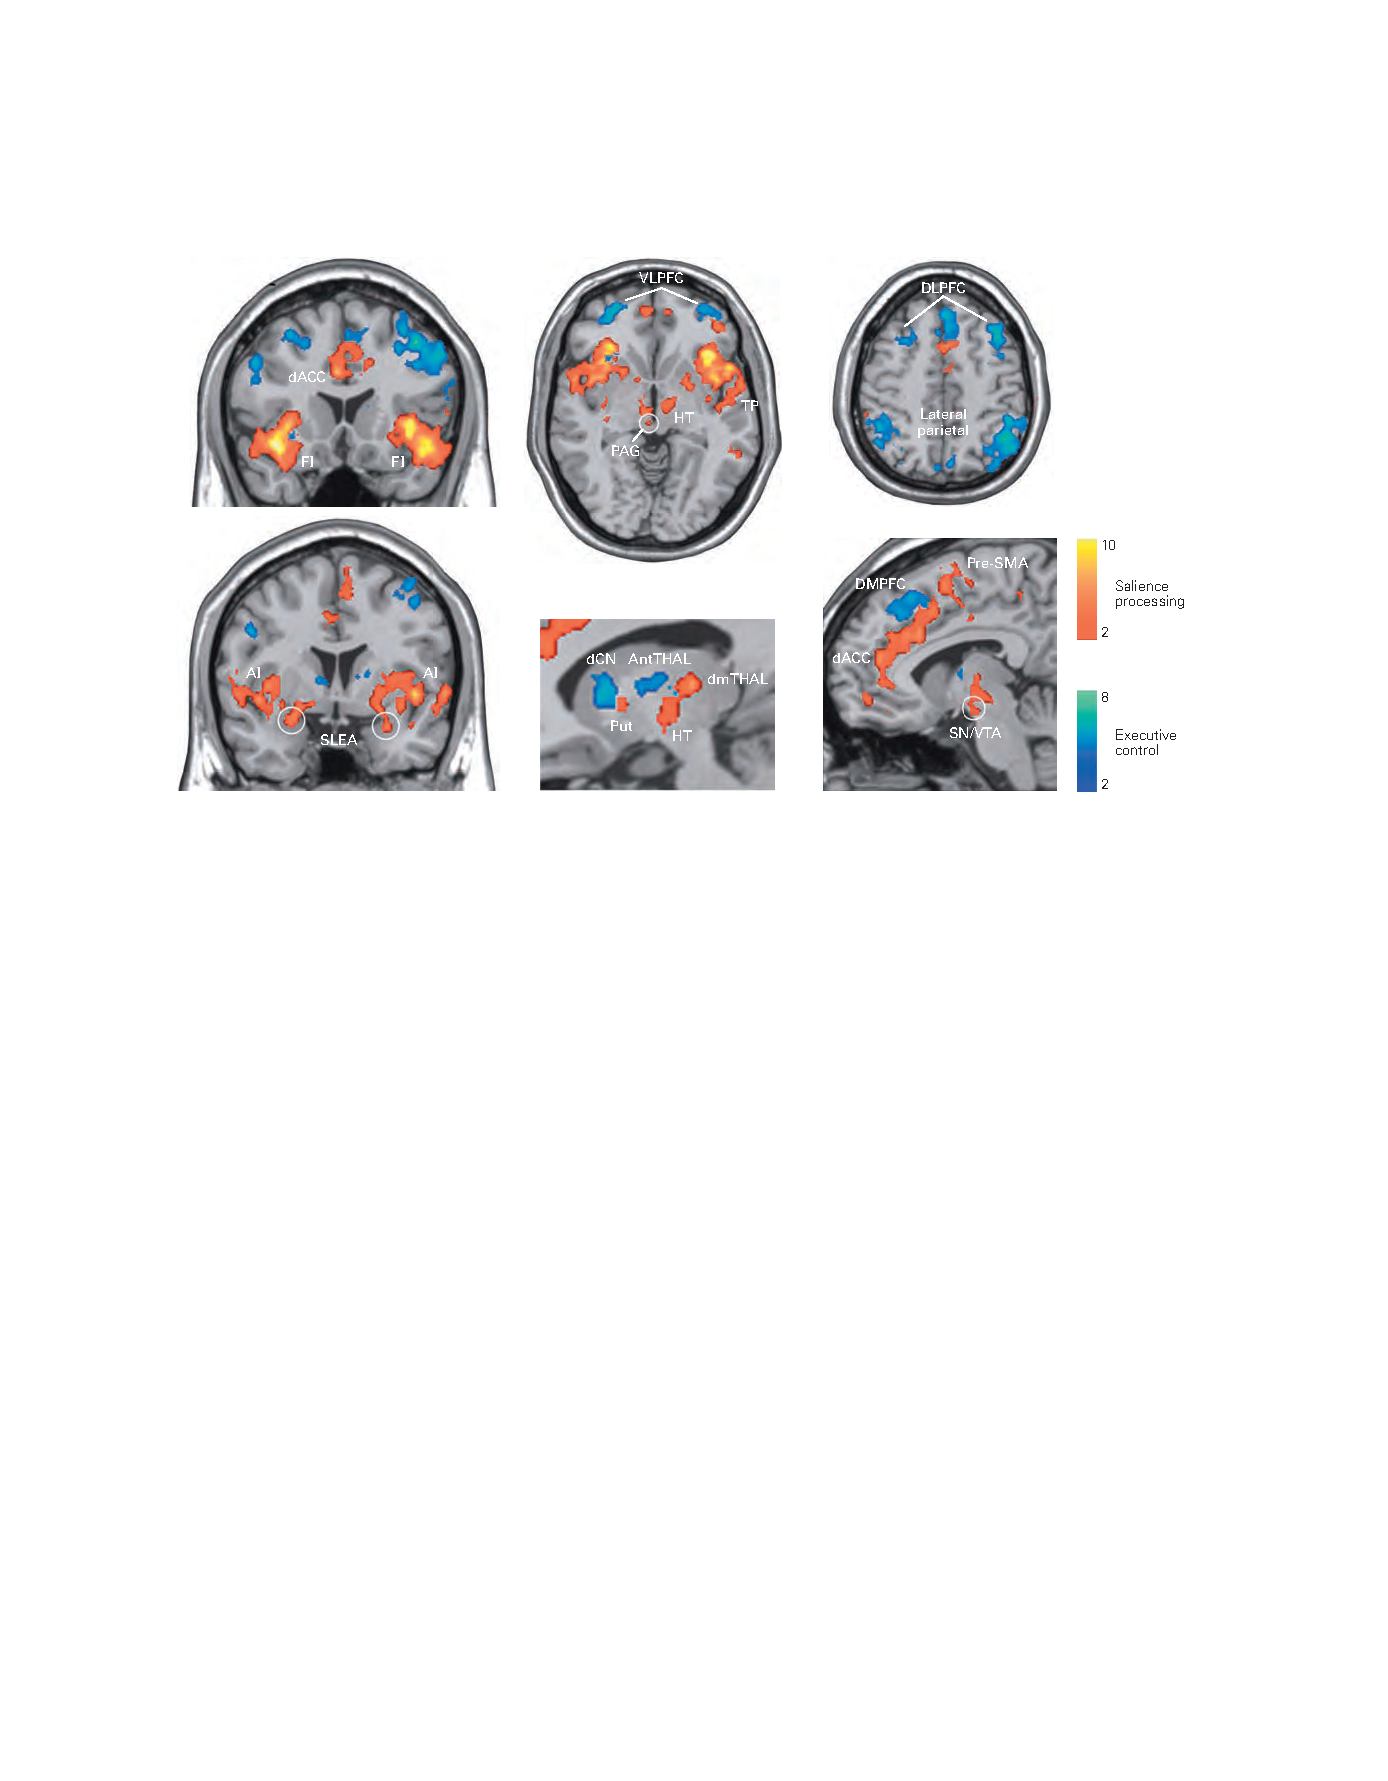
\includegraphics[width=1.0\linewidth]{chap61/fig_61_2}
	\caption{情绪障碍涉及与情绪显著性和认知控制处理相关的独立神经网络。
		应用于静息状态功能磁共振成像数据的统计分析(独立成分分析)识别出计算情绪显著性(红橙色)和调节认知控制/执行功能(蓝色)的可分离网络。
		情绪显著性网络将\textit{背前扣带皮层}和\textit{前岛叶皮层}与涉及情绪的皮层下结构联系起来。
		认知控制网络连接\textit{背外侧前额叶皮层}和顶叶皮层以及几个皮下结构。
		多项独立研究表明,本研究中显示出网络化的大脑区域与\textit{重度抑郁症}有关\cite{seeley2007dissociable}。}
	\label{fig:61_2}
\end{figure}


在健康的人类受试者中,杏仁核区域会被威胁性刺激和恐惧条件反射激活,例如将先前的中性音调与轻度电击配对。
从查尔斯达尔文的工作开始,人们已经认识到表达恐惧的人脸会在不同的人类文化中引起焦虑反应,这可能是一种在群体成员之间传达危险存在的机制。


已经在患有焦虑症或\textit{重度抑郁症}的受试者中研究了恐惧和其他表达情绪的面孔对通过\textit{功能性磁共振成像}或脑电图测量的自主神经活动和大脑活动测量的影响。
在一个这样的范例中,当受试者在核磁共振成像扫描仪中时,可怕的面孔会非常短暂地显示(33 毫秒)。
此演示文稿之后是中性面孔(称为向后遮蔽)。
在这种情况下,受试者报告说他们没有意识到看到了那张可怕的脸。
然而,它们表现出改变的皮肤电反应,一种交感神经激活的量度,以及基底杏仁核的激活,杏仁核区域处理感觉输入并对威胁做出选择性反应。
对患有创伤后应激障碍、其他焦虑症和\textit{重度抑郁症}的个体进行的几项功能性神经影像学研究表明,杏仁核活动增强,即使是无害刺激也会激活,并且与正常适应模式相比,杏仁核活动持续存在(图~\ref{fig:61_3})。


\begin{figure}[htbp]
	\centering
	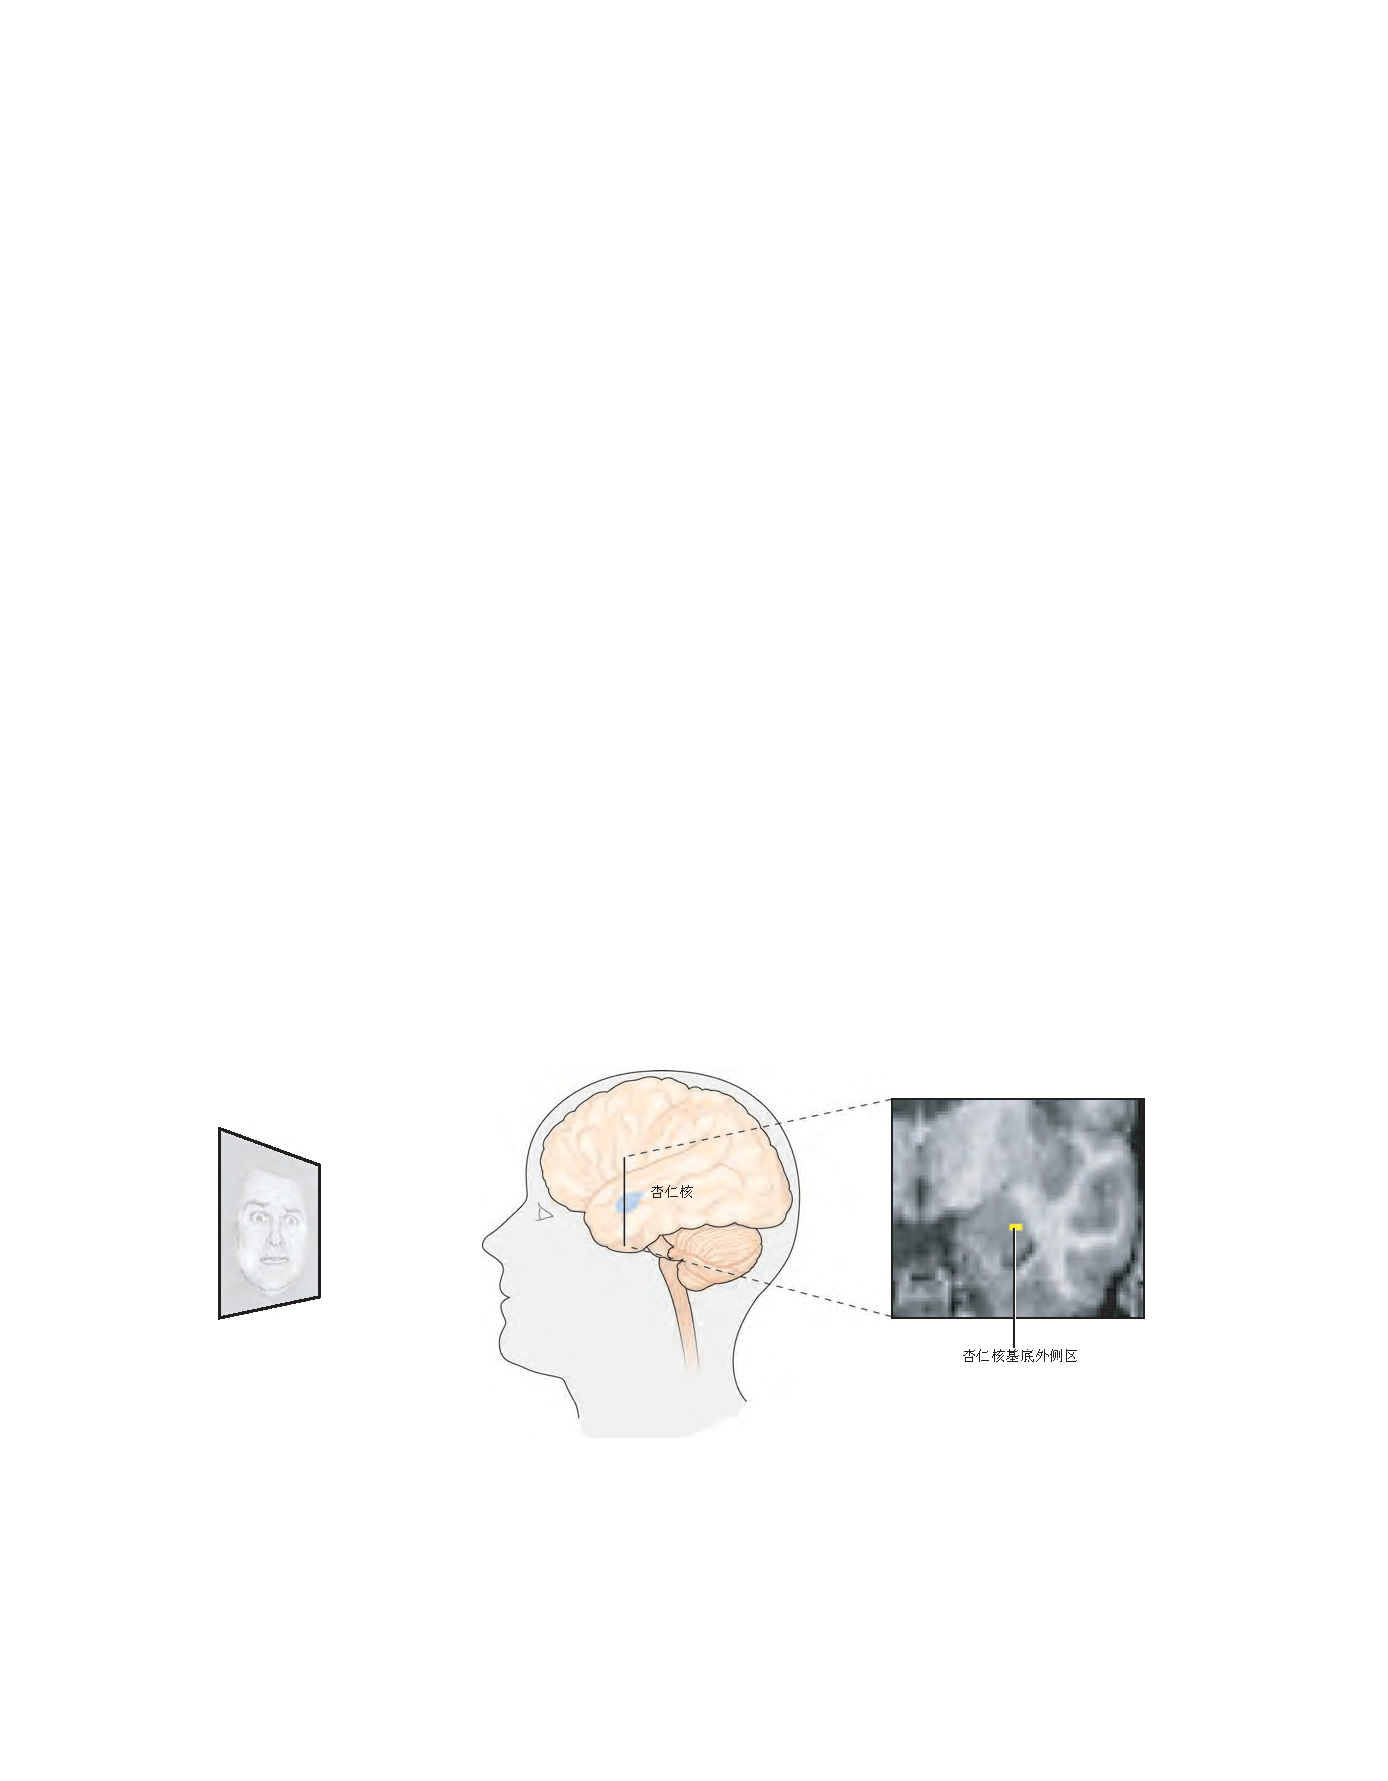
\includegraphics[width=1.0\linewidth]{chap61/fig_61_3}
	\caption{杏仁核响应可怕刺激的遮蔽呈现而激活。
		人类受试者在通过磁共振成像扫描时观察投影图像。
		当一张可怕的脸出现很短的时间,然后出现一张中性的脸时,一种称为反向遮蔽的协议,受试者不会有意识地意识到可怕的脸。
		在这些情况下,杏仁核的基底外侧区域在焦虑症患者中比在正常人中更强烈地被激活\cite{etkin2004individual}。}
	\label{fig:61_3}
\end{figure}


焦虑症和\textit{重度抑郁症}的功能性神经影像学研究还发现,与基底杏仁核相连的\textit{前额皮层}区域活动减少。
对具有\textit{前额皮层}损伤的动物的研究表明,从额叶皮层到基底杏仁核的投射对于对厌恶信息的认知控制是必要的。
在患有焦虑症或\textit{重度抑郁症}的个体中,厌恶刺激对前额叶皮层的激活减少与认知测试一致,认知测试表明认知控制下降,并可能导致过度和持续的焦虑和其他负面情绪。


\textit{重度抑郁症}和双相情感障碍的电生理学和功能性神经影像学研究表明,\textit{前扣带皮层}的前额叶皮层区域参与情绪显著性网络,其延髓侧和腹侧部分功能异常。
头侧和腹侧\textit{前扣带皮层}与海马、杏仁核、眶前额叶皮层、前岛叶和伏隔核有广泛联系,参与情绪、认知和自主神经系统功能的整合。
尾侧\textit{前扣带皮层}细分涉及与行为控制相关的认知过程;
它与前额叶皮层、次级运动皮层和后扣带皮层的背侧区域有联系。


尽管在抑郁发作中观察到\textit{前扣带皮层}两个分区的功能异常,但在\textit{重度抑郁症}和双相情感障碍的抑郁期中观察到的最一致的异常是头侧和腹侧分区的活动增加,尤其是在膝下区域腹侧胼胝体的膝。
在一项使用正电子发射断层扫描的研究中,使用选择性 5-羟色胺再摄取抑制剂抗抑郁药有效治疗\textit{重度抑郁症}与头侧\textit{前扣带皮层}活动减少相关,而健康受试者的自我诱发悲伤增加活动(图~\ref{fig:61_4})。
基于这些研究,头侧前(膝下)扣带皮层已被用作深部脑刺激电极放置的目标,以治疗难治性\textit{重度抑郁症},这在操作上被定义为对抗抑郁药物和心理治疗无反应的抑郁症。


\begin{figure}[htbp]
	\centering
	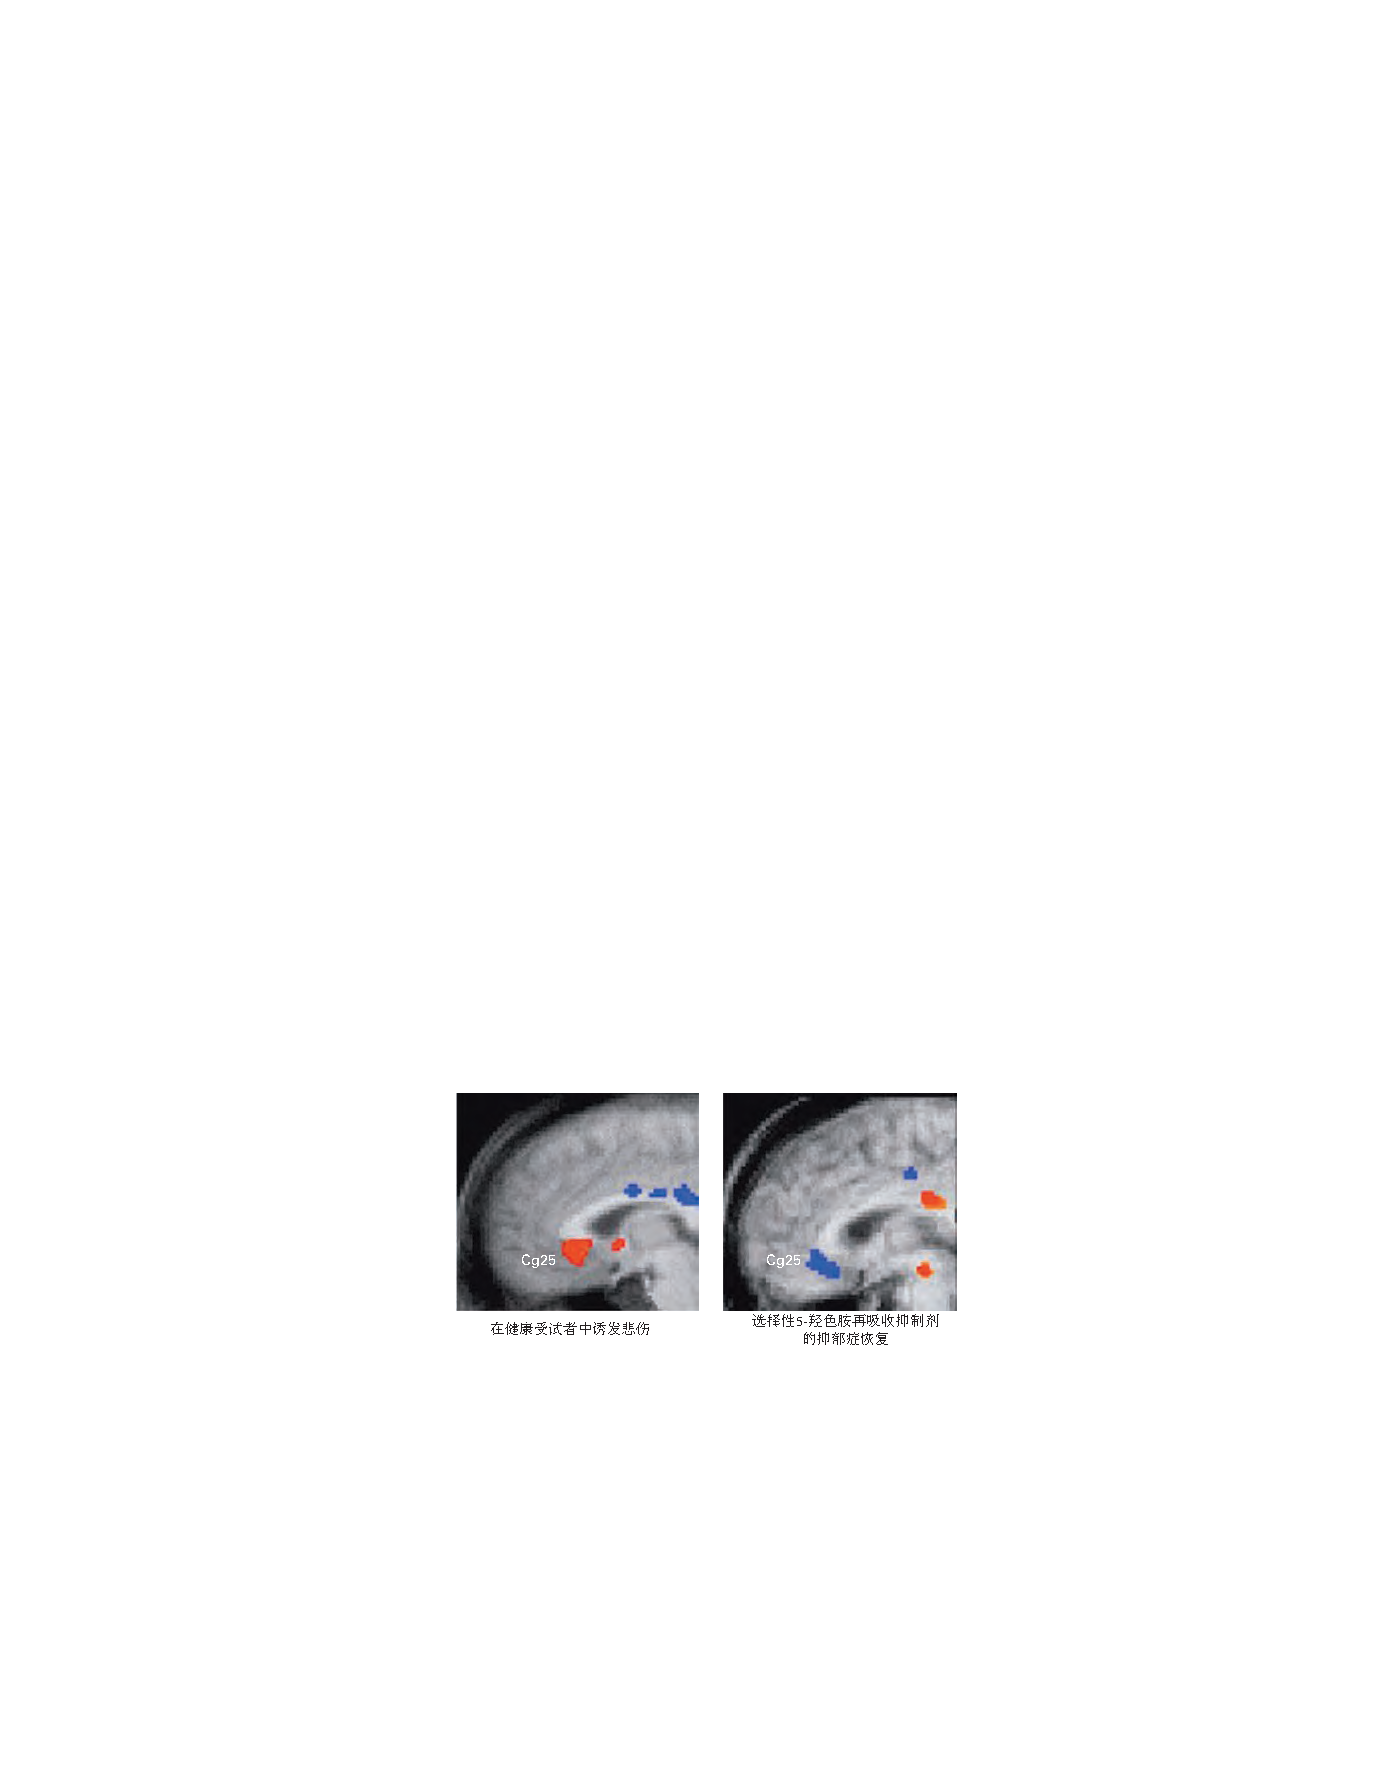
\includegraphics[width=0.7\linewidth]{chap61/fig_61_4}
	\caption{头侧前(膝下)扣带皮层的活动因悲伤而增加,因抗抑郁药成功治疗\textit{重度抑郁症}而减少\cite{mayberg1997cingulate}。
		 健康的志愿者提供了他们最悲伤记忆的脚本,后来在接受\textit{正电子发射断层成像}时用于产生短暂的悲伤。
		 当阅读悲伤的故事时,头侧\textit{前扣带皮层}被激活(人脑矢状面的红色假色)被激活。
		 \textit{正电子发射断层成像}配体是氧 15 标记的水,用于测量脑血流量作为大脑活动的代表。 正确的。
		 在患有\textit{重度抑郁症}的受试者中证实了头侧\textit{前扣带皮层}的代谢升高。
		 在使用\textit{选择性血清再吸收抑制剂}抗抑郁药成功治疗后,前\textit{布罗德曼 25 区}中的大脑活动减少(人脑矢状面呈蓝色假色)。
		 \textit{正电子发射断层成像}配体是 2-脱氧葡萄糖,用于测量大脑代谢作为大脑活动的代表。}
	\label{fig:61_4}
\end{figure}


大脑奖励回路的功能异常也可能在情绪障碍的症状中发挥作用。
奖励回路包括从中脑腹侧被盖区到前脑目标的多巴胺能投射,包括伏隔核、缰核、前额叶皮层、海马体和杏仁核(第~\ref{chap:chap43}~章)。
在正常情况下,这些途径涉及奖励的评估(例如,可口的食物、性活动和社交互动)和激励必要的行为以获得奖励。
奖励处理在抑郁症中似乎是不正常的,基于这样的症状,例如对以前愉快的活动的兴趣下降,动力下降,以及当抑郁症严重时,无法体验快乐(快感缺乏)。
尽管研究较少,但躁狂症的奖励处理也可能异常,躁狂症的特征是过度参与以目标为导向的行为,即使这些行为是不适应的,例如不受控制的支出、危险的药物使用和滥交的性活动。


在最近对静息态\textit{功能性磁共振成像}的分析中,数据显示,可以根据与快感缺乏和焦虑程度相关的连接模式对\textit{重度抑郁症}患者进行分层。
然而,尽管奖励回路的调制被认为是治疗\textit{重度抑郁症}的一种可能方法,但在实践中已被证明是困难的。
例如,已知可通过增加突触多巴胺来激活此回路的药物(如苯丙胺和可卡因)会造成过度使用和成瘾的高风险。
最近,已经开始在\textit{重度抑郁症}患者中测试从抑制控制中释放奖赏回路的药物,例如 kappa 阿片受体拮抗剂。



\subsection{海马体积的减少与情绪障碍有关}

与健康受试者相比,\textit{重度抑郁症}患者的海马体积减少是情绪障碍中最明确的结构异常。
最近对\textit{重度抑郁症}和双相情感障碍患者的研究发现,在未接受药物治疗的受试者中,与情绪控制相关的大脑皮层区域的海马体体积减少。
此类研究仍需重复,显示与双相情感障碍相比,\textit{重度抑郁症}患者的体积减少有重叠和非重叠模式。
在控制药物使用持续时间时,在\textit{重度抑郁症}患者中观察到的容量减少与抑郁发作的持续时间相关。
这些发现表明,在\textit{重度抑郁症}中,容量减少是由持续性疾病引起的,并不代表先行风险因素。
一些研究人员假设,\textit{重度抑郁症}患者皮质醇水平升高可能与海马体体积减少有关。


在创伤后应激障碍病例中也有海马体体积减少的报道。
与严重抑郁症相反,对创伤后应激障碍不一致的同卵双胞胎的研究表明,小海马先于疾病发作,因此可能代表危险因素而不是疾病的结果。


\textit{重度抑郁症}患者海马体积的获得性减少可能是由于树突和树突棘的减少,细胞数量(神经元或胶质细胞)减少,或两者兼而有之。
考虑到压力和抑郁的关系,皮质醇分泌过多可能是导致这两种损失的原因。
海马细胞数量的减少可以用压力和糖皮质激素水平升高抑制成年海马神经发生这一事实来解释,如对几种动物物种的研究所示。


在包括人类在内的几种哺乳动物中,海马齿状回内的新颗粒细胞在成年期产生。
对啮齿动物的研究表明,这些新神经元可以并入功能性神经回路中,它们最初表现出增强的结构和突触可塑性。
细胞死亡作为成人神经发生平衡的作用研究较少。


在啮齿类动物中,压力或厌恶的治疗或糖皮质激素的施用会抑制颗粒细胞前体的增殖,从而抑制海马体中神经发生的正常速率。
抗抑郁药,包括选择性血清素再摄取抑制剂,发挥相反的作用,增加神经发生的速度。
因此,抑郁症中发生的糖皮质激素应激激素的过度分泌可能会随着时间的推移抑制神经发生而导致海马体积减少。
由于海马体中的糖皮质激素受体需要对合成和释放\textit{促肾上腺皮质激素释放激素}的下丘脑神经元进行抑制性反馈,因此海马体功能受损会进一步损害\textit{下丘脑-垂体-肾上腺}轴的反馈调节,从而形成恶性循环。


海马体允许大脑解决密切相关的刺激之间的差异(模式分离),并提供有助于解释刺激的生存意义的上下文信息。
有机体需要此类信息来准确识别在复杂的感官输入流中发出的威胁信号。
在动物研究中,海马体损伤会增加焦虑反应;
人们认为,由此产生的模式分离和上下文信息处理的损害允许与威胁相关的记忆不恰当地概括,从而与无害的刺激相关联。
生理学和行为学证据表明,海马齿状回内的新生神经元在模式分离中起着特别重要的作用。
因此,抑制神经发生可能会导致通常伴随严重抑郁症的焦虑症状,而海马体积异常低可能会增加患创伤后应激障碍的风险。



\section{可以有效治疗严重的抑郁症和焦虑症}

\textit{重度抑郁症}可以通过抗抑郁药、认知心理疗法和电休克疗法得到有效治疗。
其他干预措施难以治愈的\textit{重度抑郁症}正在通过针对膝下前额叶皮层和其他目标(包括伏隔核)的深部脑刺激进行实验性治疗。



\subsection{目前的抗抑郁药物影响单胺能神经系统}

这些抗抑郁药以其第一个临床适应症命名,比其名称所暗示的具有更广泛的用途。
的确,抗抑郁药也是治疗焦虑症的一线药物。
随着风险因素和一些神经回路的频繁共现和共享,有效治疗方式的重叠进一步证明情绪和焦虑症是相关的。


所有广泛使用的抗抑郁药都会增加大脑中单胺能系统的活性,最显著的是血清素和去甲肾上腺素,尽管一些抗抑郁药也会对多巴胺产生适度的影响。
相关的单胺类神经递质(血清素、去甲肾上腺素和多巴胺)由位于脑干核内的细胞合成(第~\ref{chap:chap40}~章)。
脑桥和延髓中的 5-羟色胺能和去甲肾上腺素能神经元广泛投射到大脑区域中高度多样化的终末区域,包括下丘脑、海马体、杏仁核、基底神经节和大脑皮层(图~\ref{fig:61_5}~和~\ref{fig:61_6})。
中脑腹侧被盖区和黑质致密部的多巴胺能神经元投射到不太广泛的区域。
腹侧被盖神经元投射到海马体、杏仁核、伏隔核和前额叶皮层;
黑质神经元支配尾状核和壳核。
这些单胺能神经元广泛不同的投射使它们能够影响唤醒、注意力、警惕性、动机以及其他需要整合多个大脑区域的认知和情绪状态等功能。


\begin{figure}[htbp]
	\centering
	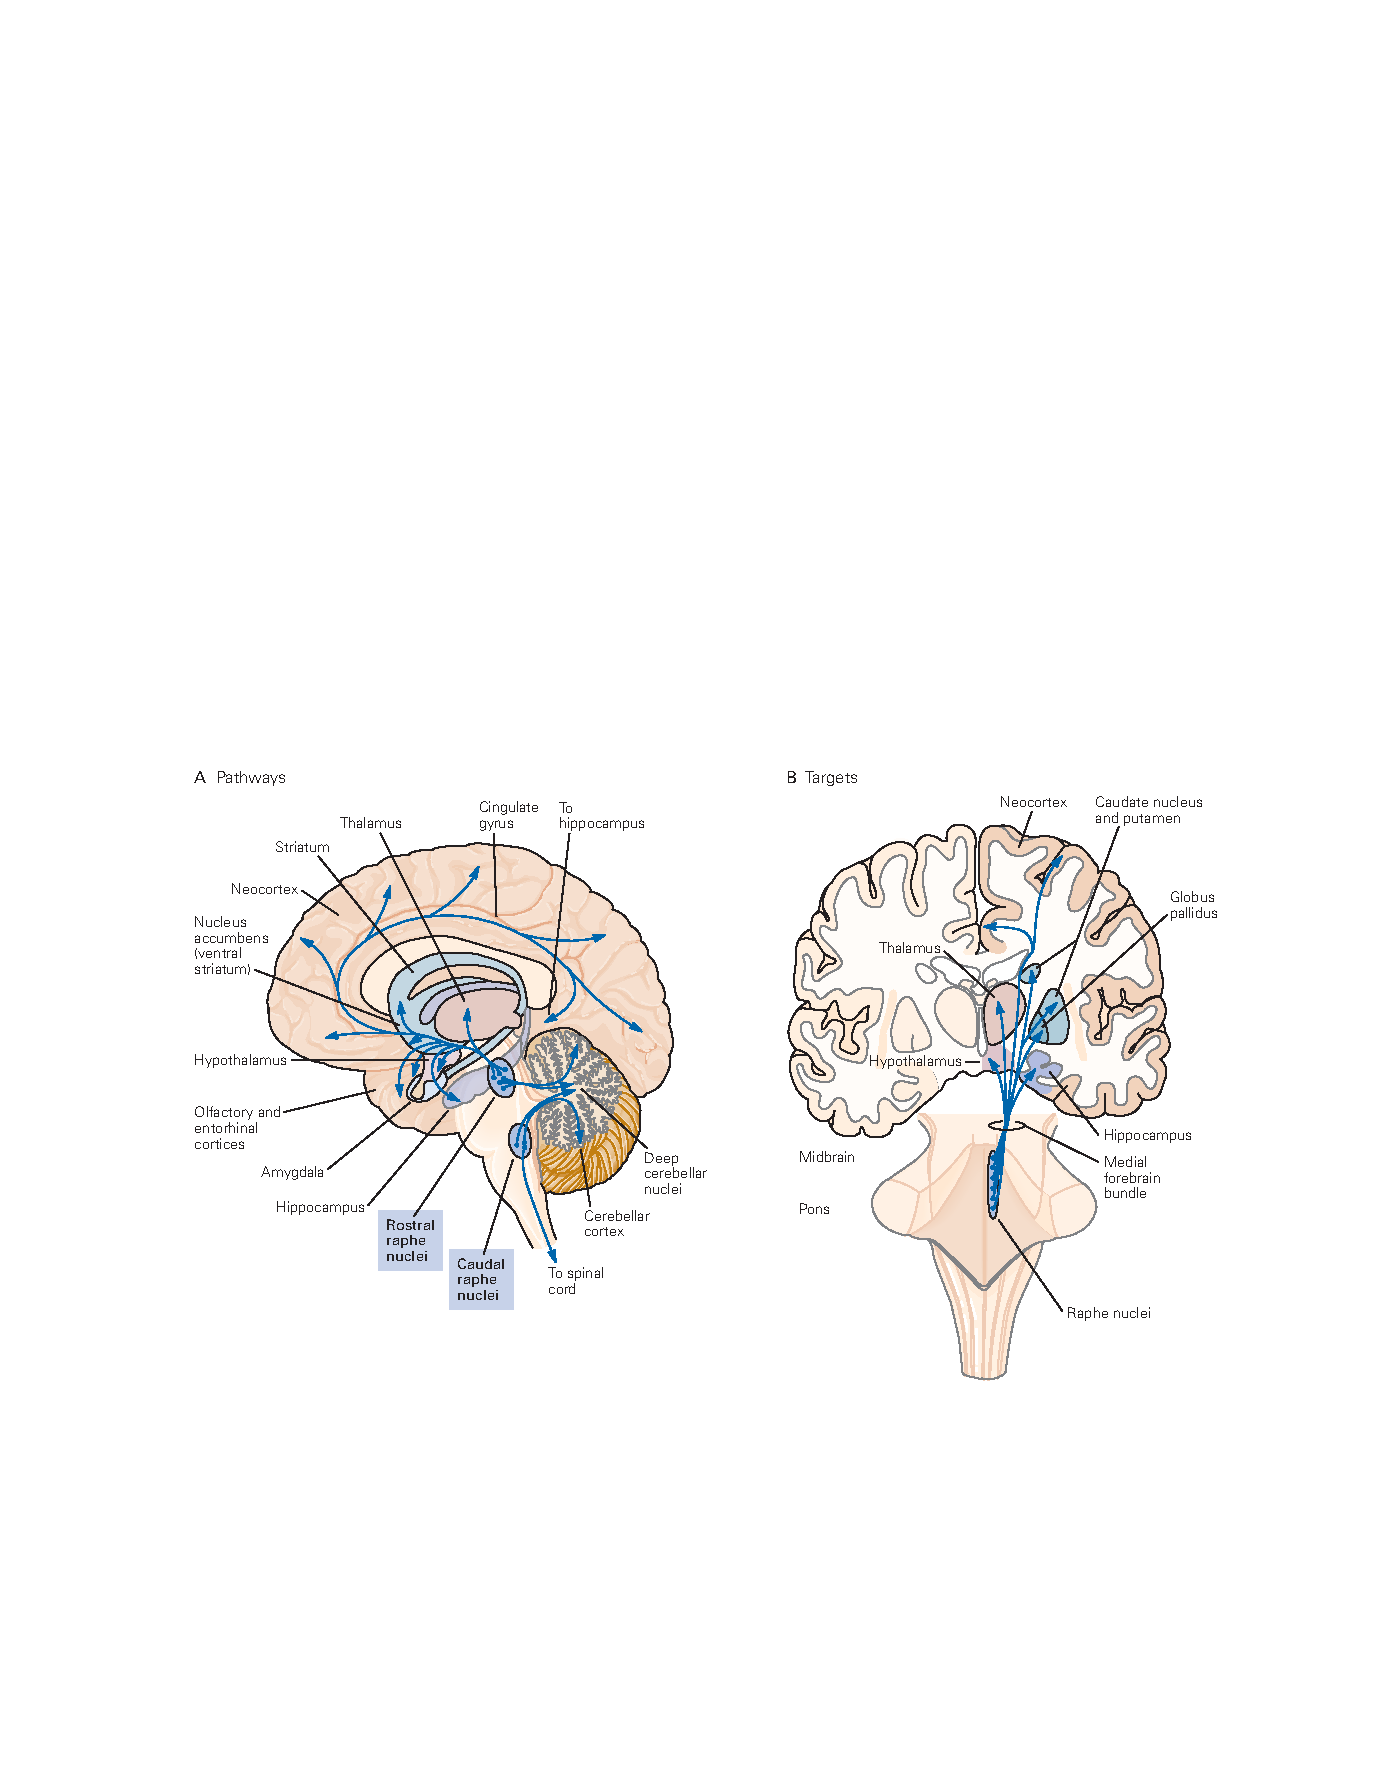
\includegraphics[width=1.0\linewidth]{chap61/fig_61_5}
	\caption{大脑中的主要血清素能系统出现在脑干的中缝核中。
		血清素在一组称为中缝核的脑干核中合成。
		这些神经元投射到整个神经轴,范围从前脑到脊髓。
		5-羟色胺能投射是单胺能系统中最庞大和最分散的,单个 5-羟色胺能神经元支配数百个目标神经元\cite{heimer2012human}。
		\textbf{A.} 大脑的矢状面图显示了中缝核。
		在大脑中,这些细胞核形成了一个相当连续的细胞群集合,靠近脑干中线并沿其长度延伸。
		在这里的图中,它们以更明显的喙部和尾部组显示。
		头侧中缝核投射到大量的前脑结构。
		\textbf{B.} 这张大脑的冠状视图说明了由血清素能中缝核神经元支配的一些主要结构。}
	\label{fig:61_5}
\end{figure}


\begin{figure}[htbp]
	\centering
	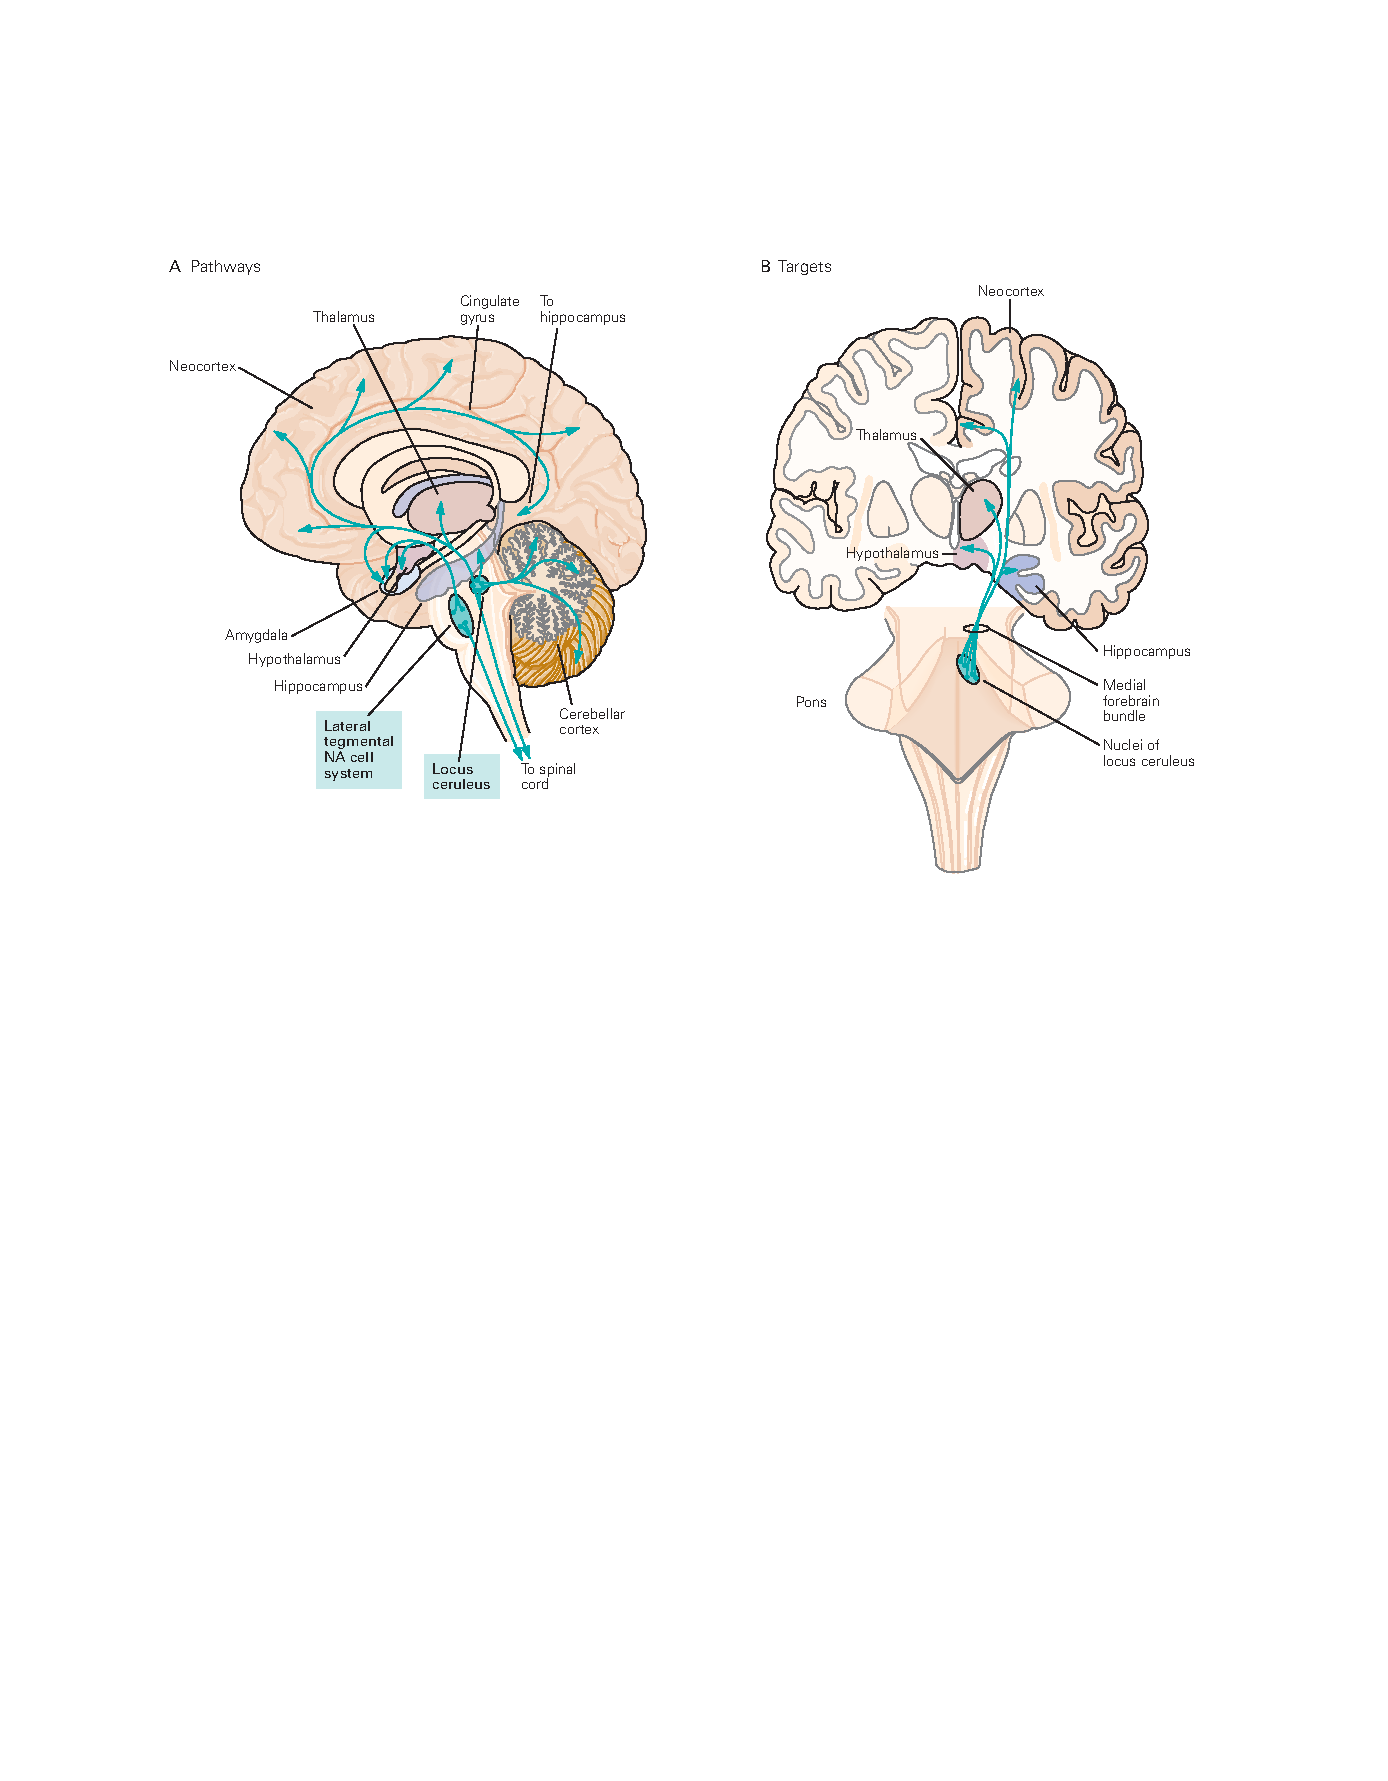
\includegraphics[width=1.0\linewidth]{chap61/fig_61_6}
	\caption{前脑的主要去甲肾上腺素能投射出现在蓝斑\cite{heimer2012human}。
		\textbf{A.} 去甲肾上腺素在几个脑干核中合成,其中最大的是蓝斑核,这是一个位于脑桥头外侧第四脑室底部正下方的色素核。
		横向正中矢状位视图显示了来自蓝斑和外侧脑干被盖的主要\textit{去甲肾上腺素能}通路的过程。
		蓝斑的轴突伸入前脑,也伸入小脑和脊髓;
		来自外侧脑干被盖区去甲肾上腺素能核的轴突投射到脊髓、下丘脑、杏仁核和腹侧前脑。
		\textbf{B.} 冠状切面显示了来自蓝斑的神经元的主要目标。}
	\label{fig:61_6}
\end{figure}


血清素、去甲肾上腺素和多巴胺由氨基酸前体合成,并包装到突触小泡中以供释放。
细胞质中位于囊泡外的单胺被\textit{单胺氧化酶}代谢,单胺氧化酶与线粒体膜的外叶相关。
囊泡释放后,单胺类神经递质结合突触受体发挥其生物学作用,或被位于突触前细胞膜上的特定转运蛋白从突触中清除。


最广泛使用的抗抑郁药分为几个主要类别,它们影响单胺能神经元及其靶点(图~\ref{fig:61_7})。
1950 年代发现的\textit{单胺氧化酶}抑制剂,如苯乙肼和反苯环丙胺,对抑郁症和焦虑症均有效,但由于其副作用,如今很少使用。
\textit{单胺氧化酶}抑制剂阻断\textit{单胺氧化酶}在突触前末梢分解去甲肾上腺素、血清素或多巴胺的能力,从而使额外的神经递质可用于包装到囊泡中并释放。


\begin{figure}[htbp] \label{fig:61_7}
	\centering
	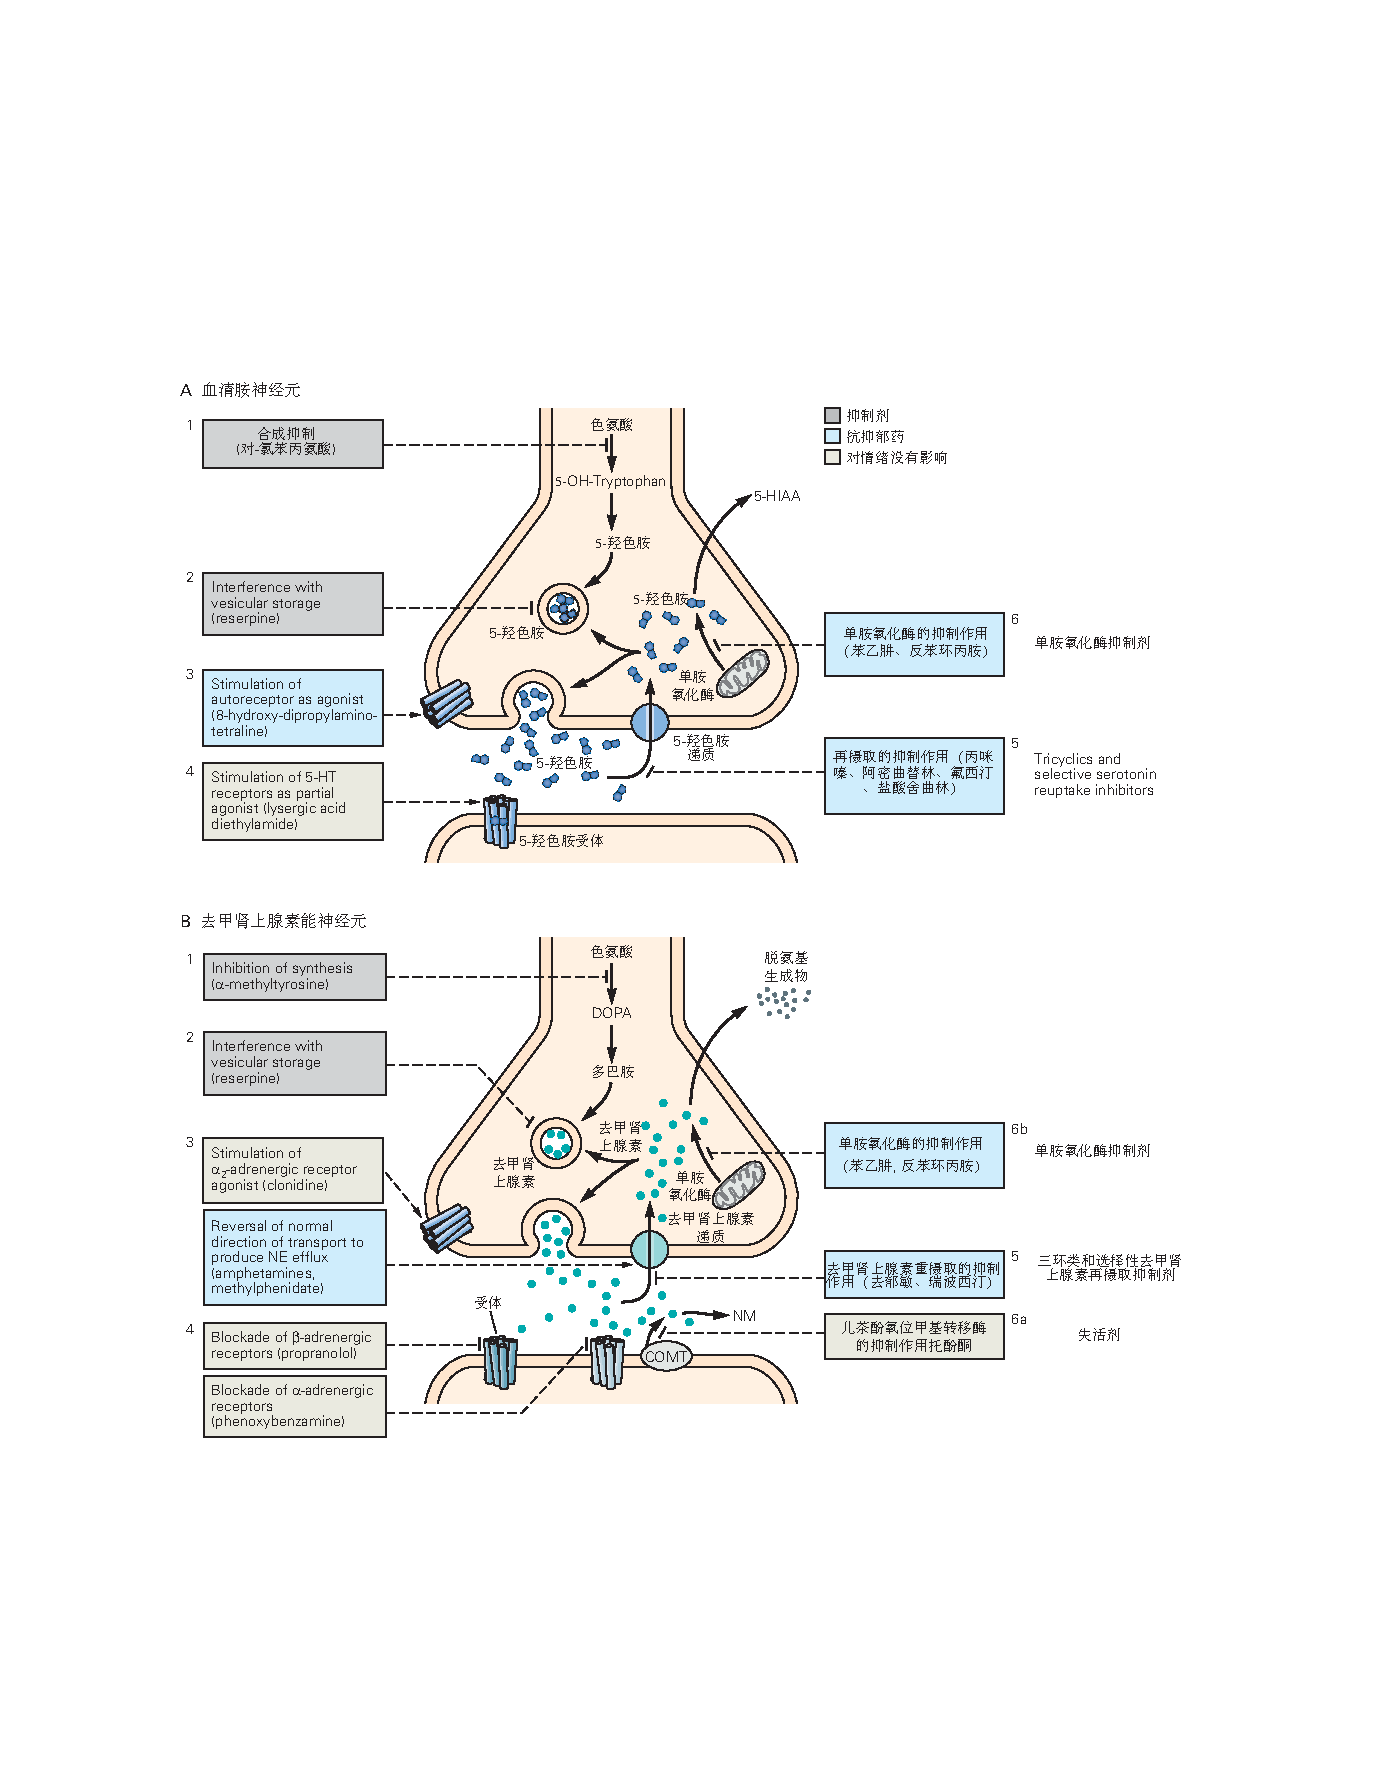
\includegraphics[width=0.63\linewidth]{chap61/fig_61_7}
	\caption{抗抑郁药在血清素能和去甲肾上腺素能突触中的作用。
	该图显示了血清素能和去甲肾上腺素能突触的突触前侧和突触后侧。
	血清素和去甲肾上腺素是通过酶促级联从氨基酸前体合成的。
	神经递质被包装在突触小泡中;
	细胞质内的游离神经递质被\textit{单胺氧化酶}代谢,单胺氧化酶是一种与突触前末梢中丰富的线粒体相关的酶。
	释放后,血清素和去甲肾上腺素与几种类型的突触前和突触后受体相互作用。
	每种神经递质都由特定的转运蛋白从突触中清除。
	血清素和去甲肾上腺素转运蛋白和\textit{单胺氧化酶}是抗抑郁药物的靶标。
	\textbf{A.} 血清素能突触的重要药物作用位点。
	图中并未显示所有描述的操作。
	1. 酶促合成。
	对氯苯丙氨酸抑制限速酶色氨酸羟化酶的合成会启动将色氨酸转化为\textit{5-羟基色氨酸}的级联反应。
	2. 储存。
	\textit{利血平}和\textit{丁苯那嗪}通过阻断囊泡单胺转运体 VMAT$_2$ 来干扰血清素和儿茶酚胺向突触囊泡的转运。
	结果,细胞质血清素被降解(见下文第 6 步),因此,神经元的神经递质被耗尽。
	利血平被用作抗高血压药物,但通常会引起抑郁症作为副作用。
	3. 突触前受体。
	突触前受体的激动剂对神经递质的合成或释放产生负反馈。
	激动剂\textit{8-羟基-二丙醇氨基-四氢萘}作用于突触前神经元上的 \textit{5-羟色氨}$_{1A}$ 受体。
	抗偏头痛曲坦类药物(如舒马普坦)是 \textit{5-羟色氨}$_{1D}$ 受体的激动剂。
	4. 突触后受体。
	致幻剂\textit{麦角酸二乙酰胺}是突触后 5-羟色胺能神经元上\textit{5-羟色氨}$_{2A}$受体的部分激动剂。
	第二代抗精神病药物,如利培酮和奥氮平,除了能够阻断 D2 多巴胺受体外,还是\textit{5-羟色氨}$_{2A}$受体的拮抗剂。
	止吐化合物昂丹司琼是 \textit{5-羟基色氨酸}3 受体的拮抗剂,\textit{5-羟基色氨酸}3 受体是单胺受体中唯一的配体门控通道。
	它的关键作用部位在髓质中。
	5. 吸收。
	选择性血清素再摄取抑制剂,如氟西汀和舍曲林,是血清素转运蛋白的选择性阻断剂。
	三环类药物混合作用;
	有些药物,如氯米帕明,对血清素转运体具有相对选择性。
	摄取阻滞剂增加血清素的突触浓度。
	苯丙胺类药物通过摄取转运蛋白进入单胺能神经元,并与突触小泡膜上的小泡转运蛋白结合,导致单胺类神经递质反向转运到细胞质中。
	然后神经递质通过摄取转运蛋白从神经元反向转运到突触中。
	6. 退化。
	苯乙肼和反苯环丙胺均对抑郁症和恐慌症有效,可阻断\textit{单胺氧化酶}-A 和 \textit{单胺氧化酶}-B。
	吗氯贝胺对抑郁症有效,对\textit{单胺氧化酶}-A 有选择性;
	已用于治疗帕金森病的司来吉兰在低剂量时对\textit{单胺氧化酶}-B 具有选择性。 
	\textbf{B.} 去甲肾上腺素能突触的重要药物作用位点。 
	1. 酶促合成。
	竞争性抑制剂 $\alpha$-甲基酪氨酸可阻断酪氨酸羟化酶催化的将酪氨酸转化为多巴的反应。
	二硫代氨基甲酸酯衍生物 FLA-63(未显示)阻断将 DOPA 转化为多巴胺的反应。
	2. 储存。
	\textit{利血平}和\textit{丁苯那嗪}通过阻断囊泡单胺转运蛋白\textit{囊泡单胺转运蛋白}干扰\textit{去甲肾上腺素}、多巴胺和血清素向突触囊泡的转运。
	结果,细胞质神经递质被降解(见下文),因此神经元的神经递质被耗尽。
	3. 突触前受体。
	突触前受体的激动剂对神经递质的合成或释放产生负反馈。
	可乐定是 $\alpha$2-肾上腺素能受体的激动剂,可抑制\textit{去甲肾上腺素}释放。
	它具有抗焦虑和镇静作用,也用于治疗注意力缺陷多动障碍。
	育亨宾是 $\alpha$2-肾上腺素能受体的拮抗剂; 它会引起焦虑。
	4. 突触后受体。
	普萘洛尔是$\beta$-肾上腺素能受体的拮抗剂,可阻断交感神经系统的许多作用。
	它用于治疗某些形式的心血管疾病,但通常用于在表演情况下阻止焦虑。
	\textit{酚苄明}是 $\alpha$-肾上腺素能受体的激动剂。
	5. 吸收。
	某些三环类抗抑郁药(如地昔帕明)和较新的\textit{去甲肾上腺素}选择性再摄取抑制剂(如瑞波西汀)选择性地阻断\textit{去甲肾上腺素}转运蛋白,从而增加突触\textit{去甲肾上腺素}。
	苯丙胺通过摄取转运蛋白进入单胺能神经元,并与囊泡转运蛋白(突触小泡上的转运蛋白)相互作用,将神经递质释放到细胞质中。
	然后神经递质通过反向作用的摄取转运体从神经元泵出进入突触。
	6. 退化。
	在突触后神经元,托酚酮抑制\textit{儿茶酚氧位甲基转移酶},从而使\textit{去甲肾上腺素}失活(步骤 6a)。
	\textit{去甲肾上腺素}是由\textit{儿茶酚氧位甲基转移酶}对\textit{去甲肾上腺素}的作用形成的。
	在突触前神经元,\textit{单胺氧化酶}的降解被 \textit{单胺氧化酶}抑制剂苯乙肼和反苯环丙胺阻断。}
\end{figure}


在大脑中发现了两种形式的\textit{单胺氧化酶},A 型和 B 型。
A 型也存在于肠道和肝脏中,它分解代谢食物中存在的生物活性胺。
\textit{单胺氧化酶}-A 的抑制作用允许生物活性胺(如酪胺)从含有高浓度它的食物(如陈年肉类和奶酪)进入血液。
转运蛋白将这些胺穿梭到交感神经元的末端,在那里它们可以将内源性囊泡去甲肾上腺素和肾上腺素置换到细胞质中,导致非囊泡释放,从而导致血压显著升高。


三环类抗抑郁药也是在 20 世纪 50 年代中期首次发现的,包括丙咪嗪、阿米替林和地昔帕明;
它们会阻断\textit{去甲肾上腺素转运蛋白}、\textit{血清素再摄取转运蛋白}或两者。
这些药物可有效治疗抑郁症和焦虑症。
然而,除了它们的治疗目标外,较老的三环类药物还会阻断许多神经递质受体,包括毒蕈碱乙酰胆碱、组胺 H1 和 $\alpha$1 去甲肾上腺素能受体,从而产生一系列副作用。


氟西汀、舍曲林和帕罗西汀等\textit{选择性血清再吸收抑制剂}于 1980 年代首次获得批准,其疗效并不比较早的三环类抗抑郁药和\textit{单胺氧化酶}抑制剂强,但被广泛使用,因为它们的副作用较轻,并且如果使用更安全 服用过量。
顾名思义,它们会选择性地抑制\textit{血清素再摄取转运蛋白}。
它们对\textit{重度抑郁症}和许多焦虑症有效。
在高剂量下,选择性血清素再摄取抑制剂对强迫症的症状也有效。
选择性去甲肾上腺素和 5-羟色胺-去甲肾上腺素再摄取抑制剂也已开发出来;
这些药物具有与选择性 5-羟色胺再摄取抑制剂相似的副作用特征,但对某些不能从单独抑制\textit{血清素再摄取转运蛋白}中获益的患者有用。


尽管了解介导抗抑郁药物、\textit{单胺氧化酶}或单胺转运蛋白作用的初始分子靶标,但它们缓解抑郁症的最终分子机制仍然未知。
理解这些药物的治疗作用的一个主要挑战是它们治疗效果的延迟。
尽管抗抑郁药在首次给药时结合并抑制\textit{单胺氧化酶}、\textit{去甲肾上腺素转运蛋白}或\textit{血清素再摄取转运蛋白},但通常需要数周的治疗才能观察到抑郁症状的解除。


已经提出了几个假设来解释这种延迟。
一个是新合成蛋白质的缓慢积累会以治疗抑郁症的方式改变神经元的反应能力。
另一个是血清素或去甲肾上腺素突触传递水平的增加会迅速增加不同情绪处理回路的可塑性,而治疗效果的延迟反映了新体验改变突触权重所需的时间。
第三个假设是抗抑郁功效部分是通过增强海马神经发生来介导的。
由于缺乏良好的抑郁症动物模型,缩小可能的治疗机制具有挑战性。
如果没有动物模型,就不可能知道许多可观察到的分子、细胞和突触变化中的哪一个会导致抑郁症或有效抗抑郁药治疗作用的基础。



\subsection{氯胺酮显示出作为治疗\textit{重度抑郁症}的快速起效药物的前景}

氯胺酮可阻断\textit{N-甲基-D-天冬氨酸}谷氨酸受体,目前用于儿科麻醉,因为它能够产生解离体验和镇痛作用。
它已经在患有严重抑郁症的受试者的随机临床试验中进行了研究。
在试验中,氯胺酮通过静脉输注给药;
它在 2 小时内产生抗抑郁作用,与通常需要数周才能显示疗效的现有抗抑郁药物相比具有显著优势。
氯胺酮的治疗效果持续约 7 天,此后第二和第三剂可能继续有效。
如果这样的结果得到广泛复制,氯胺酮将成为第一种不对单胺神经传递发挥主要作用的抗抑郁药。
确定氯胺酮缓解抑郁症的机制的研究,就像那些较老的抗抑郁药一样,具有挑战性,部分原因是缺乏良好的抑郁症动物模型。


在较高剂量下,氯胺酮被滥用为娱乐性药物,会产生欣快感、解离感、人格解体和幻觉。
氯胺酮也被用于实验室环境中,以在人类受试者中诱发让人联想到精神分裂症的认知症状。
尽管速效抗抑郁药的优势很明显,例如在治疗有严重自杀倾向的个体方面,但氯胺酮有害的精神作用使其使用存在问题。
正在尝试开发替代的\textit{N-甲基-D-天冬氨酸}受体阻断剂,其中抗抑郁作用可能与精神副作用分开。



\subsection{心理疗法可有效治疗\textit{重度抑郁症}和焦虑症}

针对抑郁症和焦虑症开发了短期的以症状为中心的心理疗法,并在临床试验中进行了测试。
研究得最好的心理疗法是认知行为疗法。
可用于治疗\textit{重度抑郁症}的认知疗法侧重于识别和纠正对事件和与他人互动的过度负面解释。
例如,许多抑郁症患者对负面信息表现出强烈的注意力偏见,自动将中性事件解释为负面,并将不赞成他人行为的证据读入。
这种可以引发或延续抑郁情绪的自动消极思维可以通过认知心理疗法得到很大改善。


具有更多行为成分的疗法已被证明可用于治疗焦虑症,例如恐惧症或创伤后应激障碍。
在暴露疗法中,受影响的个体被引导生动地回忆起引发焦虑或回避的恐惧刺激。
治疗师为此类体验提供安全的环境,并建议对此类刺激进行新的解释,以帮助患者应对这种体验。
在可能且患者可以忍受的情况下,可以采用逐渐过渡到现实世界暴露于恐惧刺激的方法。


暴露疗法产生类似于动物行为研究的消退学习。
对恐惧刺激的记忆并没有被抹去,但是恐惧反应被新的信息所抑制,即刺激和经历它的环境并不危险。
动物生理学和损伤研究以及人类成像研究表明,前额叶皮层是消退学习所必需的,而海马体是学习熟悉事件或刺激的新环境所必需的(例如,直升机从头顶飞过并不预示着攻击)。



\subsection{电休克疗法对抑郁症非常有效}

尽管它在大众的想象中仍然会让人联想到负面形象,但现代麻醉下的\textit{电痉挛疗法}在医学上是安全的,并且患者体验可以接受,并且它仍然是严重\textit{重度抑郁症}急性治疗的高效干预措施。
它最常用于抑郁症状严重且药物和心理治疗无效的情况。
它对双相情感障碍的抑郁期和躁狂期也有效。
在没有情绪障碍的情况下,它对焦虑症无效,并且不用于临床治疗。


通常,会进行六到八次治疗,最常见的是在门诊进行。
患者被麻醉,电刺激刚好高于阈值,以产生全身性癫痫发作的脑电图证据。
主要的副作用是不同程度的顺行性和逆行性遗忘症。
通过单侧放置电极并使用所需的最低水平电刺激,可以最大限度地减少但不能消除失忆症。
给予\textit{电痉挛疗法}的啮齿动物表现出神经递质的大量释放,这导致基因表达的显著激活,可能导致大规模的神经可塑性。
然而,参与治疗反应的精确分子、细胞和回路仍然未知。



\subsection{正在开发新形式的神经调节来治疗抑郁症}

正在探索其他形式的大脑治疗性电刺激,其动机是希望改善\textit{电痉挛疗法}的治疗效果,同时减少其副作用。
这些方法通常被描述为“神经调节”。


\textit{经颅磁刺激}在头皮上使用一种装置来传递快速交替磁刺激的短暂脉冲。
这会诱导电流在设备下方大脑皮层区域的轴突内流动。
每天对左前额叶皮层进行\textit{经颅磁刺激}是安全且有效的,已获得美国食品和药物管理局的监管批准。
尽管如此,在随后的试验中,它的功效似乎并不大。
旨在提高疗效的其他临床实验正在进行中。


正在开发的替代疗法包括磁癫痫发作疗法,这是一种\textit{电痉挛疗法}的替代方法,其中磁场用于产生癫痫发作。
这种实验性疗法的希望是重现\textit{电痉挛疗法}的疗效,同时减少顺行和逆行遗忘。


上文提到的\textit{脑深部电刺激}是一种侵入性神经调节治疗,广泛用于治疗帕金森病和特发性震颤的运动症状。
为了治疗帕金森病,通常将电极放置在丘脑底核内,丘脑底核是参与运动控制的基底神经节回路的一个组成部分,与调节情绪的回路相比,这一点已广为人知。
\textit{脑深部电刺激}电极由一根导线连接,该导线从头骨伸出并在头皮和颈部皮肤下行进,连接到位于胸部的控制器和电池组,就像心脏起搏器的电池一样。
电极刺激其目标的速率可以从外部控制,通常由治疗团队调整以优化治疗反应。
在过去十年中,\textit{脑深部电刺激}的临床试验已从帕金森病和其他运动障碍扩展到精神疾病。
除了用于治疗难治性抑郁症外,\textit{脑深部电刺激}正在研究用于治疗强迫症。


大脑中的几个位置已成为\textit{脑深部电刺激}治疗抑郁症的目标。
如图~\ref{fig:61_4}~所述,头侧前(膝下)扣带皮层被悲伤激活。
因此,它已被用作难治性抑郁症的\textit{脑深部电刺激}靶点(图~\ref{fig:61_8})。
在一些临床系列中,60\% 的治疗耐药患者通过刺激膝下扣带皮层实现稳定改善。
但是,无法在大型多站点临床试验中复制使用该目标的相似水平的疗效。
患者选择的差异、大脑解剖学的个体差异或电极放置的微小差异可能是迄今为止所见不同结果的原因。
简而言之,抑郁症具有高度异质性,单一的\textit{脑深部电刺激}目标并不适用于所有难治性患者也就不足为奇了。


\begin{figure}[htbp]
	\centering
	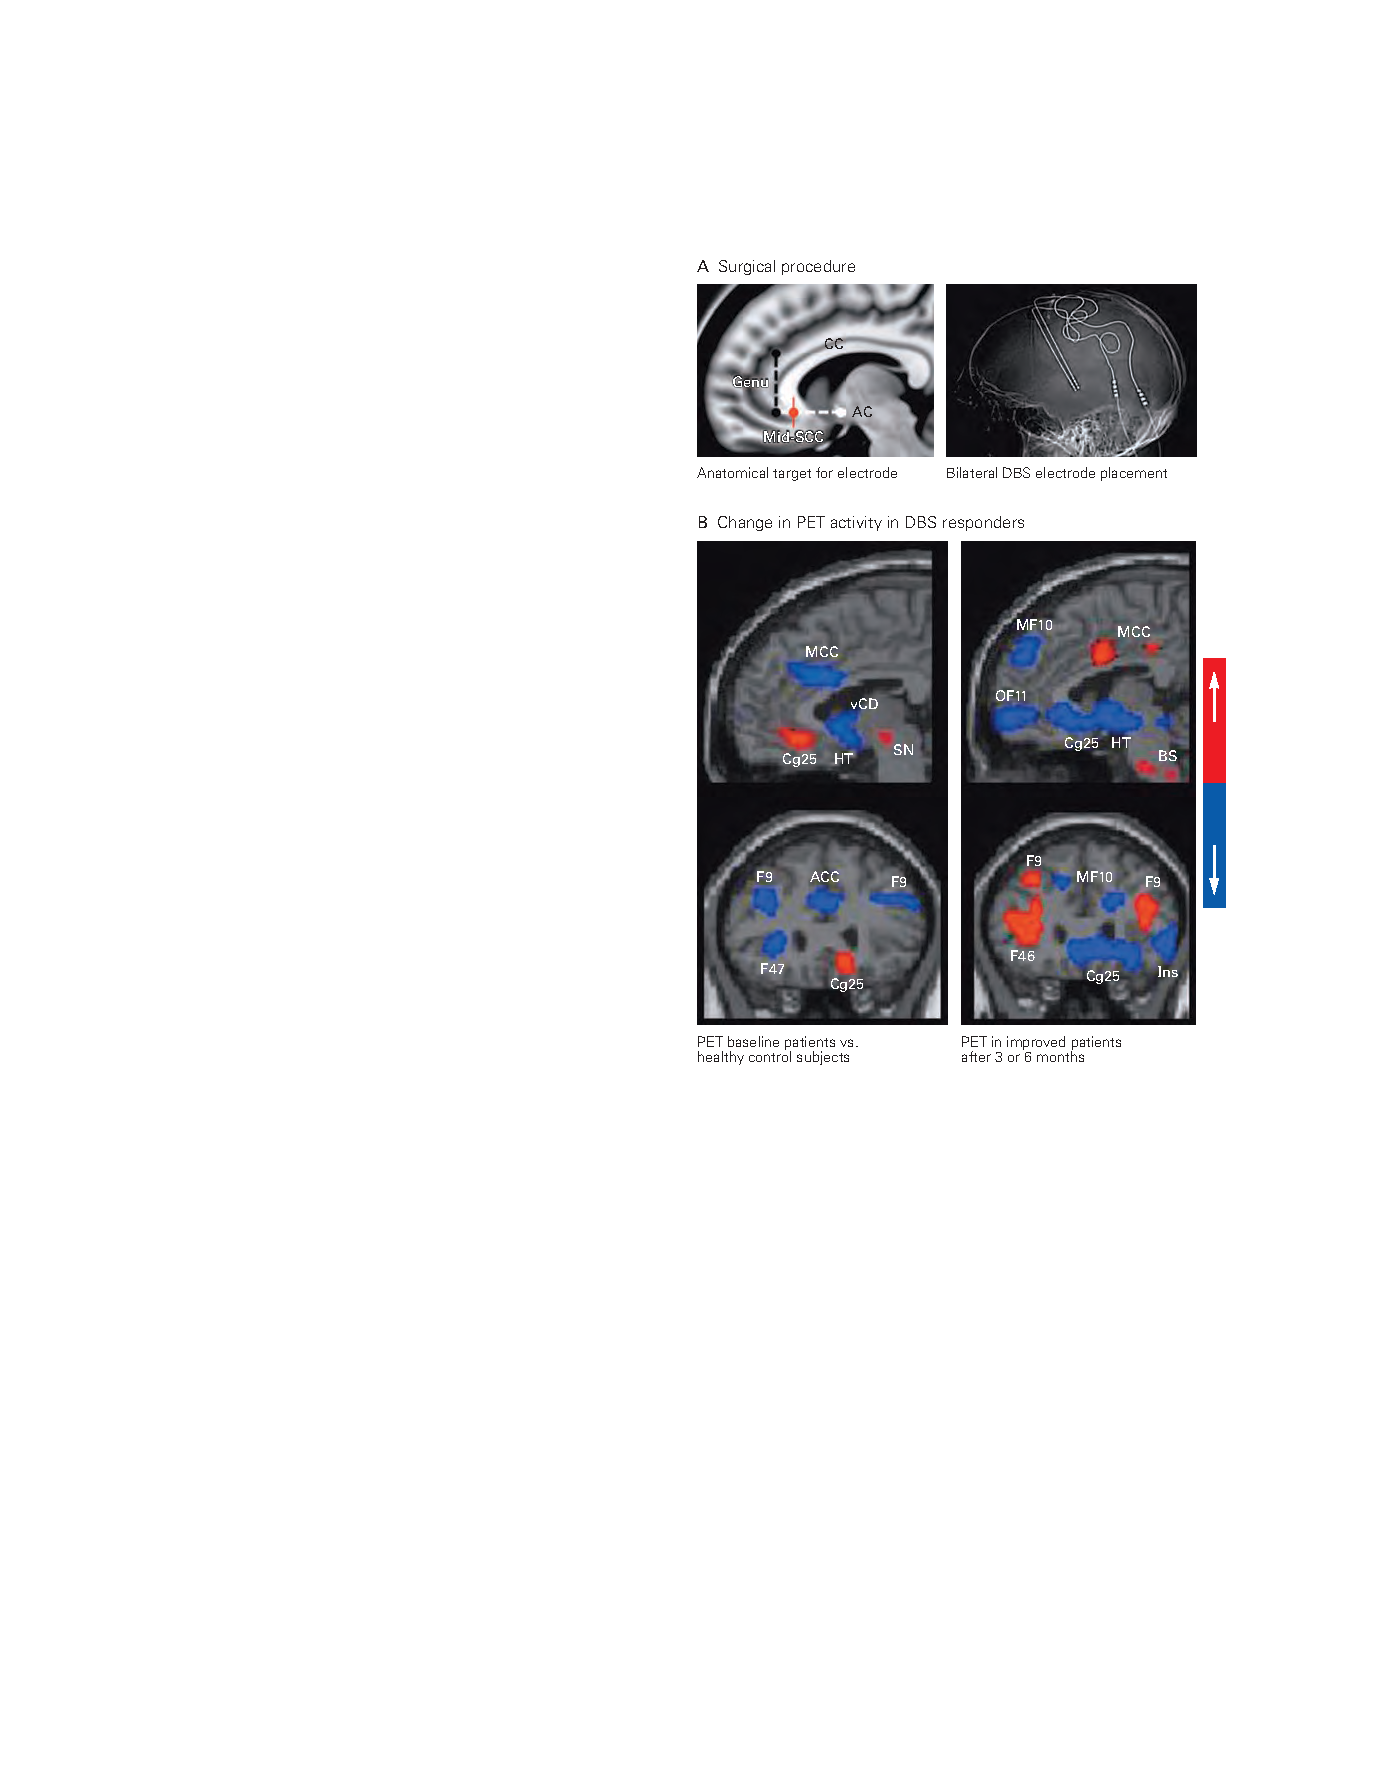
\includegraphics[width=1.0\linewidth]{chap61/fig_61_8}
	\caption{头侧\textit{前扣带皮层}\textit{脑深部电刺激}的电极放置以及通过 [18F] 氟-2-脱氧葡萄糖\textit{正电子发射断层成像}测量的反应。
		\textbf{A.} 左:头侧前(膝下)扣带皮层,布罗德曼 25 区,是难治性抑郁症患者\textit{脑深部电刺激}的解剖学目标。
		(矢状切面;红色电极部位;胼胝体刚好在上部并以白色显示;虚线,电极相对于 AC-膝线的位置。)
		右图:\textit{正电子发射断层成像}扫描显示电极在接受头侧前扣带回皮层刺激的患者大脑中的位置。 (矢状切面。)
		\textbf{B.} \textit{正电子发射断层成像}扫描显示患有难治性抑郁症的患者的活动变化,这些患者在刺激头侧\textit{前扣带皮层}后有所改善。
		上图是矢状切面;
		底部面板是冠状剖面。
		左图:难治性抑郁症患者治疗前的代谢活动。 红色假色表示与健康对照受试者相比代谢活动升高(注意\textit{脑深部电刺激}前\textit{布罗德曼 25 区}的活动升高); 蓝色表示较低的代谢活动。
		右:开始\textit{脑深部电刺激}后 3 或 6 个月改善的患者的平均值。
		在对刺激有积极反应的患者中,前\textit{布罗德曼 25 区}的活性降低(蓝色)。}
	\label{fig:61_8}
\end{figure}


由于缺乏良好的情绪障碍动物模型,人类\textit{脑深部电刺激}治疗试验可能会提供有关导致精神障碍症状的大脑回路的特别重要的信息来源。
尽管必须特别注意获得知情同意和安全,特别是当患者的判断受到严重抑郁症的影响时,\textit{脑深部电刺激}可能提供学习情绪调节的机会。
特别是,新开发的电极不仅可以刺激\textit{脑深部电刺激}目标,还可以记录细胞外神经元活动。
这种“读写”电极目前仅用于研究环境,它不仅可以改善临床结果,还可以提高我们对回路功能障碍和精神疾病治疗调节的认识。



\subsection{第二代抗精神病药物是双相情感障碍的有效治疗方法}

所有抗精神病药物均通过阻断 D2 多巴胺受体起作用,但这些药物早已被认为不仅在治疗精神分裂症、严重情绪障碍和许多其他病症的精神病症状方面具有治疗作用,而且在治疗急性躁狂症方面也具有治疗作用 剧集。
第一代抗精神病药物的副作用很严重,最突出的是 D2 多巴胺受体拮抗作用导致的帕金森样运动副作用。


大多数第二代药物对 D2 多巴胺受体的亲和力略低于第一代药物,此外,还具有其他受体作用,例如阻断\textit{5-羟基色氨酸}A 受体,从而降低严重运动副作用的可能性。
这些药物绝非没有严重的副作用;
大多数会导致体重增加和相关的代谢状况。
然而,它们的相对耐受性和它们对 5-羟色胺受体的影响使它们成为双相情感障碍抑郁期和急性躁狂症的重要治疗方法。
它们在治疗学中发挥了重要作用,因为双相抑郁症比单相抑郁症更不可能对抗抑郁药物产生反应。



\section{亮点}

1. 情绪障碍根据抑郁症是否单独发生(单相)或一个人是否同时患有躁狂发作,分为单相障碍和双相障碍。
单相和双相障碍具有不同的家族传播模式。 


2.临床上显著的单相抑郁症,常被称为\textit{重度抑郁症},它与正常悲伤的区别在于它的持续性、普遍性,以及与生理、认知和行为症状的关联。


3. \textit{重度抑郁症}很常见(终生患病率为 15\%–20\%)并致残,使其成为全世界致残的主要原因。
双相情感障碍不太常见(全世界终生患病率为 1\%),但往往会产生严重的症状,通常需要住院治疗。 


4. 焦虑症是最常见的精神疾病。
它们的严重程度从恐慌症和创伤后应激障碍的高度致残病例到简单的恐惧症不等。
他们经常与\textit{重度抑郁症}同时发生。


5. 情绪障碍和焦虑障碍既有遗传风险也有非遗传风险。
双相情感障碍比\textit{重度抑郁症}或焦虑症更容易遗传。
童年逆境和后来的环境压力因素在\textit{重度抑郁症}和焦虑症的易感性中起着重要作用。
双相情感障碍、\textit{重度抑郁症}和创伤后应激障碍的遗传分析开始产生发病机制的分子线索。


6. 恐惧和焦虑症的神经回路涉及杏仁核及其与\textit{前额皮层}的相互联系。
\textit{重度抑郁症}和双相情感障碍的神经回路不太清楚。
然而,患有\textit{重度抑郁症}的人的神经影像学涉及涉及情绪显著性处理和认知控制的回路。


7.双相情感障碍可以用锂盐、某些抗惊厥药物如丙戊酸和第二代抗精神病药物治疗,尽管许多患者有残留症状,最常见的是抑郁症。


8. 严重的抑郁症和焦虑症可以用多种抗抑郁药以及认知和行为疗法来治疗。
电休克疗法对对药物无反应的\textit{重度抑郁症}有效。


9. 正在研究用于治疗\textit{重度抑郁症}和其他精神疾病的深部脑刺激等实验疗法。
可以记录和刺激的电极的开发有望更深入地了解人类神经回路在疾病及其治疗中的功能。




